%
% This work is licensed under a Creative Commons Attribution-ShareAlike 4.0 International License.
% http://creativecommons.org/licenses/by-sa/4.0/
%
\documentclass{beamer}
\usetheme[pageofpages=of,% String used between the current page and the
                         % total page count.
          bullet=circle,% Use circles instead of squares for bullets.
          titleline=true,% Show a line below the frame title.
          alternativetitlepage=true,% Use the fancy title page.
	  titlepagelogo=images/logoM-circl-Forensics.png,% Logo for the first page.
%          watermark=watermark-polito,% Watermark used in every page.
%          watermarkheight=100px,% Height of the watermark.
%          watermarkheightmult=4,% The watermark image is 4 times bigger
                                % than watermarkheight.
          ]{Torino}

\usepackage[utf8]{inputenc}
\usepackage{listings}
\usepackage{color}
\usepackage[font=small,labelfont=bf]{caption}
\usepackage{transparent}
\usepackage{siunitx}

\usepackage[norndcorners,customcolors]{hf-tikz}
\hfsetbordercolor{yellow}
\hfsetfillcolor{yellow}

\lstset{ 
  backgroundcolor=\color{white},   % choose the background color; you must add \usepackage{color} or \usepackage{xcolor}
  basicstyle=\footnotesize,        % the size of the fonts that are used for the code
  breakatwhitespace=false,
}


\author{CIRCL \emph{TLP:WHITE}}
\title{CIRCL - DFIR 1.0.2}
\subtitle{Introduction: File System Forensics and Data Recovery}
\institute{info@circl.lu}
\date{Edition May 2020}



\begin{document}
\begin{frame}[t,plain]
\titlepage
\end{frame}

\begin{frame}
  \frametitle{Thanks to:}
  \begin{itemize}
  \item[] AusCERT
    \begin{figure}
        
\includegraphics[scale=0.3, angle=0, trim=0 0 0 0]{images/auscert_logo.png}
    \end{figure}
  \item[] JISC
    \begin{figure}
        
\includegraphics[scale=0.06, angle=0, trim=0 0 0 0]{images/jisc-logo.png}
    \end{figure}
  \end{itemize}
\end{frame}


\begin{frame}
  \frametitle{Overview}
  \begin{itemize}
  \item[]
      \begin{enumerate}
          \item File System Analysis - Overview
          \item FAT - File Allocation Table
          \item NTFS - New Technology File System
          \item NTFS - Advanced
          \item File System Time Line
          \item Carving
          \item String Search
          \item Forensics Challenges
          \item Bibliography and Outlook
      \end{enumerate}
  \end{itemize}
\end{frame}


%
% This work is licensed under a Creative Commons Attribution-ShareAlike 4.0 International License.
% http://creativecommons.org/licenses/by-sa/4.0/
%

% DO NOT COMPILE THIS FILE DIRECTLY!
% This is included by the other .tex files.


\begin{frame}
    
\includegraphics[scale=0.3]{images/logo-circl-Forensics.png}
    \begin{itemize}
        \item[]
        \item[]
        \item[] 1. File System Analysis - Overview
    \end{itemize}
\end{frame}


\begin{frame}[fragile]
  \frametitle{1.1 Abstract: Components of a file system}
  \begin{lstlisting}[basicstyle=\tiny\ttfamily]
             File System: - Organize data on a block device
			  - Maintain an allocation table
                          - Utilize meta data
                            
        ---------------------------------------------
        |                   |                       |
        V                   V                       V

    File Name            Metadata                Content     
-----------------    -----------------       ---------------------------------- ...
| file1.txt     |    |Time stamps,   | 13    |................................| 5001
| -> Inode: 13  |    |Owner, Group,  |       |................................| 5002
|---------------|    |Rights: MACB,  |       |....                            | 5003
| file2.txt     |    |5001,5002,5003 |       |................................| 5004
| -> Inode: 14  |    |Size: 68 Byte  |       |.......................         | 5005
|---------------|    |---------------|       |                                | 5006
| file3.txt     |    |Time stamps,   | 14    |                                | ...
| -> Inode: xyz |    |Owner, Group,  |       |                                | ...
|---------------|    |Rights: MACB,  |       |                                | ...
| ............  |    |5004,5005      |       |                                | ...
| ............  |    |Size: 55 Byte  |       |      ( 32 Byte cluster )       | 5011
-----------------    -----------------       ---------------------------------- ...
                     | ............  |        |       |       |       |      |
                     | ............  |        0       8      16      24     31
                     -----------------    

Allocation table (Meta): 13, 14
       Allocation table: 5001, 5002, 5003, 5004, 5005
  \end{lstlisting}
\end{frame}


\begin{frame}[fragile]
  \frametitle{1.2 Delete a file: Allocated $\to$ Unallocated}
  \begin{lstlisting}[basicstyle=\tiny\ttfamily]
             File System: - Organize data on a block device
			  - Maintain an allocation table
                          - Utilize meta data
                            
        ---------------------------------------------
        |                   |                       |
        V                   V                       V

    File Name            Metadata                Content     
-----------------    -----------------       ---------------------------------- ...
| file1.txt     |    |Time stamps,   | 13    |................................| 5001
| -> Inode: 13  |    |Owner, Group,  |       |................................| 5002
|---------------|    |Rights: MACB,  |       |....                            | 5003
| file2.txt XX  |    |5001,5002,5003 |       |................................| 5004
| -> Inode: 14  |    |Size: 68 Byte  |       |.......................         | 5005
|---------------|    |---------------|       |                                | 5006
| file3.txt     |    |Time stamps,   | 14    |                                | ...
| -> Inode: xyz |    |Owner, Group,  |       |                                | ...
|---------------|    |Rights: MACB,  |       |                                | ...
| ............  |    |5004,5005      |       |                                | ...
| ............  |    |Size: 55 Byte  |       |      ( 32 Byte cluster )       | 5011
-----------------    -----------------       ---------------------------------- ...
                     | ............  |        |       |       |       |       |
                     | ............  |        0       8      16      24     31
                     -----------------    

Allocation table (Meta): 13
       Allocation table: 5001, 5002, 5003
  \end{lstlisting}
\end{frame}


\begin{frame}[fragile]
  \frametitle{1.3 Slack space}
  \begin{lstlisting}[basicstyle=\tiny\ttfamily]
   ----------------------------------------------------------------------------
   +    +    +    |    +    +    +    |    +    +    +    |    +    +    +    |
   ----------------------------------------------------------------------------

                  |                   |                   |                   |
                  |                   |                   |                   |

                  -------------------------------------------------------------
                  |....+....+....+....|....+..00+????+????|                   |
                  -------------------------------------------------------------
                            1                   1                   0 

0 = Unallocated
1 = Allocated


Evolution of slack space:
-------------------------
	- Complete cluster is allocated to the file
	- Until end of sector: Filled with zeros (or random memory --> RAM slack)
	- Until end of cluter: Don't touch at all --> File slack
	- Maybe there are rests of deleted file content.
  \end{lstlisting}
\end{frame}


\begin{frame}[fragile]
  \frametitle{1.4 Metadata based file recovery: Abstract}
  \begin{lstlisting}[basicstyle=\tiny\ttfamily]
1. Create file: file1.txt

    File Name              Inode                 Content     
-----------------    -----------------       ---------------------------------- ...
| file1.txt     |    |7123, 7124     | 13    |                                | 7122
| -> Inode: 13  |    |.....          |       |  H e l l o                     | 7123
|---------------|    |---------------|       |  W o r l d                     | 7124
| ............  |    |               | 14    |                                | ...
| ............  |    |               |       |                                | ...
-----------------    -----------------       ---------------------------------- 
                     | ............  |
		     | ............  |       Allocation table (Meta): 13
                     -----------------              Allocation table: 7123, 7124


2. Delete file: file1.txt

    File Name              Inode                 Content     
-----------------    -----------------       ---------------------------------- ...
| file1.txt XX  |    |7123, 7124     | 13    |                                | 7122
| -> Inode: 13  |    |.....          |       |  H e l l o                     | 7123
|---------------|    |---------------|       |  W o r l d                     | 7124
| ............  |    |               | 14    |                                | ...
| ............  |    |               |       |                                | ...
-----------------    -----------------       ---------------------------------- 
                     | ............  |
		     | ............  |       Allocation table (Meta): 14
                     -----------------              Allocation table: 7122, 7123
  \end{lstlisting}
\end{frame}


\begin{frame}[fragile]
  \frametitle{1.4 Metadata based file recovery: Abstract}
  \begin{lstlisting}[basicstyle=\tiny\ttfamily]
2. Delete file: file1.txt

    File Name              Inode                 Content     
-----------------    -----------------       ---------------------------------- ...
| file1.txt XX  |    |7123, 7124     | 13    |                                | 7122
| -> Inode: 13  |    |.....          |       |  H e l l o                     | 7123
|---------------|    |---------------|       |  W o r l d                     | 7124
| ............  |    |               | 14    |                                | ...
| ............  |    |               |       |                                | ...
-----------------    -----------------       ---------------------------------- 
                     | ............  |
		     | ............  |       Allocation table (Meta): 
                     -----------------              Allocation table: 


3. Create file: file2.txt (Partially overwrite data of file1.txt)

    File Name              Inode                 Content     
-----------------    -----------------       ---------------------------------- ...
| file1.txt XX  |    |7123, 7124     | 13    |  T h i s   i s                 | 7122
| -> Inode: 13  |    |.....          |       |  P a u l a                     | 7123
|---------------|    |---------------|       |  W o r l d                     | 7124
| file2.txt     |    |7122, 7123     | 14    |                                | ...
| -> Inode: 14  |    |               |       |                                | ...
-----------------    -----------------       ---------------------------------- 
                     | ............  |
		     | ............  |       Allocation table (Meta): 14
                     -----------------              Allocation table: 7122, 7123
  \end{lstlisting}
\end{frame}


\begin{frame}[fragile]
  \frametitle{1.4 Metadata based file recovery: Abstract}
  \begin{lstlisting}[basicstyle=\tiny\ttfamily]
3. Create file: file2.txt (Partially overwrite data of file1.txt)

    File Name              Inode                 Content     
-----------------    -----------------       ---------------------------------- ...
| file1.txt XX  |    |7123, 7124     | 13    |  T h i s   i s                 | 7122
| -> Inode: 13  |    |.....          |       |  P a u l a                     | 7123
|---------------|    |---------------|       |  W o r l d                     | 7124
| file2.txt     |    |7122, 7123     | 14    |                                | ...
| -> Inode: 14  |    |               |       |                                | ...
-----------------    -----------------       ---------------------------------- 
                     | ............  |
		     | ............  |       Allocation table (Meta): 14
                     -----------------              Allocation table: 7122, 7123


 

  # Recovery of a (deleted) file
  $ dd if=deleted.dd of=file2.txt bs=32 skip=7122 count=2
            --> This is Paula

  
  # Recovery of a reallocated file
  $ dd if=deleted.dd of=file1.txt bs=32 skip=7123 count=2
            --> Paula World


  Discussion: What did we miss in this abstract example?
  \end{lstlisting}
\end{frame}


\begin{frame}[fragile]
  \frametitle{1.5 The Sleuth Kit}
  \begin{lstlisting}[basicstyle=\tiny\ttfamily]
  mmstat	# Volume system information
  mmls		# List partition table
  mmcat		# Cat a partition

  fsstat	# File system information

  fls		# List files and directories
  fcat		# Cat a file
  ffind		# Find filename of an inode

  istat		# Inode information
  ils		# List inodes
  icat		# Cat an inode
  ifind		# Find inode of a sector

  blkstat	# Information of a data unit
  blkls		# Output data units
  blkcat	# Cat a data unit

  jls		# List content of journal
  jcat		# Cat a block from journal

  mactime	# File system time line
  srch_strings	# Display printable characters
  hfind		# Hash database lookup
  ....
  \end{lstlisting}
\end{frame}


\begin{frame}[fragile]
  \frametitle{1.6 Metadata based file recovery: The Sleuth Kit}
  \begin{lstlisting}[basicstyle=\tiny\ttfamily]
3. Create file: file2.txt (Partially overwrite data of file1.txt)

    File Name              Inode                 Content     
-----------------    -----------------       ---------------------------------- ...
| file1.txt XX  |    |7123, 7124     | 13    |  T h i s   i s                 | 7122
| -> Inode: 13  |    |.....          |       |  P a u l a                     | 7123
|---------------|    |---------------|       |  W o r l d                     | 7124
| file2.txt     |    |7122, 7123     | 14    |                                | ...
| -> Inode: 14  |    |               |       |                                | ...
-----------------    -----------------       ---------------------------------- 
                     | ............  |
		     | ............  |       Allocation table (Meta): 14
                     -----------------              Allocation table: 7122, 7123



  # Recovery of a (deleted) file
  $ icat deleted 14 > file2.txt
            --> This is Paula
 

  # Recovery of a reallocated file
  $ icat deleted 13 > file1.txt
            --> Paula World
  \end{lstlisting}
    \begin{itemize}
        \item[] Exercise: Recover deleted files from \texttt{/carving/deleted.dd}
    \end{itemize}
\end{frame}


\begin{frame}[fragile]
  \frametitle{1.7 File slack and unallocted clusters}
    \begin{itemize}
	    \item Slack: Manual approach with \texttt{dd}
  \begin{lstlisting}[basicstyle=\tiny]
fsstat deleted.dd
    Cluster Size: 4096

fls -r deleted.dd

istat deleted.dd 72
    size: 12071
    1131 1132 1133

$ echo $(( (3*4096) - 12071 ))
  217

dd if=deleted.dd bs=4096 skip=1133 count=1 | xxd | less 
  \end{lstlisting}
	    \item Slack: Automated approach with The Sleuthkit
  \begin{lstlisting}[basicstyle=\tiny]
blkls -s -b 4096 usb.dd
  \end{lstlisting}
	    \item Exercise: Does file recovery incl. slack?
	    \item Blocks: With The Sleuthkit
  \begin{lstlisting}[basicstyle=\tiny]
blkls -a -b 4096 deleted.dd | xxd | less              # Allocated blocks
blkls -A -b 4096 deleted.dd | xxd | less              # Unallocated blocks
blkls -e -b 4096 deleted.dd | xxd | less              # All blocks
  \end{lstlisting}
    \end{itemize}
\end{frame}






%
% This work is licensed under a Creative Commons Attribution-ShareAlike 4.0 International License.
% http://creativecommons.org/licenses/by-sa/4.0/
%

% DO NOT COMPILE THIS FILE DIRECTLY!
% This is included by the other .tex files.


\begin{frame}
    
\includegraphics[scale=0.3]{images/logo-circl-Forensics.png}
    \begin{itemize}
        \item[]
        \item[]
        \item[] 2. FAT - File Allocation Table
    \end{itemize}
\end{frame}


\begin{frame}[fragile]
  \frametitle{2.1 FAT file system structure}
    \begin{itemize}
	    \item Layout and VBR Example
  \begin{lstlisting}[basicstyle=\tiny]
--------------------------------
|      Volume Boot Record      |     0000: eb3c 906d 6b66 732e 6661 7400 0204 0400
--------------------------------     0010: 0200 0200 00f8 4000 2000 4000 0000 0000
|             FAT1             |     0020: 0000 0100 8000 2974 6812 e84e 4f20 4e41
--------------------------------     0030: 4d45 2020 2020 4641 5431 3620 2020 0e1f
|             FAT2             |     0040: be5b 7cac 22c0 740b 56b4 0ebb 0700 cd10
--------------------------------     0050: 5eeb f032 e4cd 16cd 19eb fe54 6869 7320
|   Root Directory (FAT12/16)  |     .....
--------------------------------
|                              |
|                              |     Exercise: fat16.dd = 33.554.432 Byte
|         Data Clusters        |     Can you calculate the size or this FAT16?
|                              |
|                              | 
--------------------------------
  \end{lstlisting}
	    \item VBR interpretation
  \begin{lstlisting}[basicstyle=\tiny]
Offset      Length   Item             Interpretation
00 (0x00)   3        Jump bootstrap   JMP 62 NOP
03 (0x03)   8        OEM name         mkfs.fat
11 (0x0B)   2        Bytes/sector     0x0002 --> 0x0200 =  512 Bytes
13 (0x0D)   1        Sectors/Cluster  0x04              = 2048 Bytes
14 (0x0E)   2        Sector before FS 0x0400 --> 0x0004 =    4 Sectors
16 (0x10)   1        Copies of FAT    0x02
.....
  \end{lstlisting}
    \end{itemize}
\end{frame}


\begin{frame}[fragile]
  \frametitle{2.1 FAT Filesystem structures}
    \begin{itemize}
	    \item Layout and VBR Example
  \begin{lstlisting}[basicstyle=\tiny]
--------------------------------
|      Volume Boot Record      |     0000: eb3c 906d 6b66 732e 6661 7400 0204 0400
--------------------------------     0010: 0200 0200 00f8 4000 2000 4000 0000 0000
|             FAT1             |     0020: 0000 0100 8000 2974 6812 e84e 4f20 4e41
--------------------------------     0030: 4d45 2020 2020 4641 5431 3620 2020 0e1f
|             FAT2             |     0040: be5b 7cac 22c0 740b 56b4 0ebb 0700 cd10
--------------------------------     0050: 5eeb f032 e4cd 16cd 19eb fe54 6869 7320
|   Root Directory (FAT12/16)  |     .....
--------------------------------
|                              |
|                              |     Exercise: fat16.dd = 33.554.432 Byte
|         Data Clusters        |     Can you calculate the size or this FAT16?
|                              |
|                              |     Solution: 33554432 / 512 / 4 * 2 /  512
--------------------------------     
  \end{lstlisting}
	    \item VBR interpretation                      
  \begin{lstlisting}[basicstyle=\tiny]
Offset      Length   Item             Interpretation
00 (0x00)   3        Jump bootstrap   JMP 62 NOP
03 (0x03)   8        OEM name         mkfs.fat
11 (0x0B)   2        Bytes/sector     0x0002 --> 0x0200 =  512 Bytes
13 (0x0D)   1        Sectors/Cluster  0x04              = 2048 Bytes
14 (0x0E)   2        Sector before FS 0x0400 --> 0x0004 =    4 Sectors
16 (0x10)   1        Copies of FAT    0x02
.....
  \end{lstlisting}
    \end{itemize}
\end{frame}


\begin{frame}[fragile]
  \frametitle{2.2 FAT components simplified}
  \begin{lstlisting}[basicstyle=\tiny]
Root Directory:                         |       Content of file:  
                                        |                                  
     Name     Ext    Start   Size       |       Not part of Root directory
    -----------------------------       |       ----------------------------
     file_A   txt        3     28       |       aaaaaaaaaaaaaaaaaaaaaaaaaaaa
     file_B   txt        7      4       |       bbbb
          .....                                                             
                                                                             
                                                                             
Data Clusters: (Size of 8 characters)
     -------------------------------------------------------------------------
     |        |aaaaaaaa|aaaaaaaa|aaaaaaaa|        |bbbb    |        |        |
     -------------------------------------------------------------------------
            0        1        2        3        4        5        6        7  
     -------------------------------------------------------------------------
     |        |        |aaaa    |        |        |        |        |        |
     -------------------------------------------------------------------------
            8        9        A        B        C        D        E        F

  
FAT: FAT16 in this example                                                 
     -----------------------------------------------------------------------
     |f8ff|ffff|0000|0004|0005|000C|0000|ffff|0000|0000|0000|0000|ffff|0000|
     -----------------------------------------------------------------------
        0    1    2    3    4    5    6    7    8    9    A    B    C    D
       Reserved 
  \end{lstlisting}
\end{frame}


\begin{frame}[fragile]
  \frametitle{2.3 FAT Filesystems}
    \begin{itemize}
	    \item Examine the FAT16
  \begin{lstlisting}[basicstyle=\tiny]
fsstat FAT/fat16.dd
     .....
     Total Range: 0 - 65535
     * Reserved: 0 - 3
     ** Boot Sector: 0
     * FAT 0: 4 - 67
     * FAT 1: 68 - 131
     * Data Area: 132 - 65535
     ** Root Directory: 132 - 163
     ** Cluster Area: 164 - 65535
     .....
     Sector Size: 512
     Cluster Size: 2048
     Total Cluster Range: 2 - 16344
  \end{lstlisting}
	    \item Test files:
  \begin{lstlisting}[basicstyle=\tiny]
     5000 Nov 27 14:21 file01.txt
       50 Nov 28 10:38 file02.txt

file01.txt
     .....AAAAAAAAAAAAAAAAAAAAAAAAAAAAAAAAAAAA.....
  
file02.txt
     .....XXXXXXXXXXXXXXXXXXXXXXXXXXXXXXXXXXXX.....
  
\end{lstlisting}
    \end{itemize}
\end{frame}


\begin{frame}[fragile]
  \frametitle{2.4 FAT file system analyzed}
  \begin{lstlisting}[basicstyle=\tiny]
Root Directory: dd if=FAT/fat16.dd skip=132 count=1 | xxd | less

     0020: 4649 4c45 3031 2020 5458 5420 0064 c46a  FILE01  TXT .d.j
     0030: 7b4d 7b4d 0000 c46a 7b4d 0300 8813 0000  {M{M...j{M......
     .....
     0060: 4649 4c45 3032 2020 5458 5420 0064 104d  FILE02  TXT .d.M
     0070: 7c4d 7c4d 0000 104d 7c4d 0600 3200 0000  |M|M...M|M..2...
 
     Offset      Length   Item             Interpretation
     00 (0x00)   11       File Name        FILE01  TXT
     .....
     26 (0x1A)    2       Low Cluster      0x0300 --> 03
     28 (0x1C)    4       Size in Byes     0x8813 --> 0x1388 == 5000


Data Clusters:

     dd if=FAT/fat16.dd skip=164 count=4 | xxd | less    ................
     dd if=FAT/fat16.dd skip=168 count=4 | xxd | less    AAAAAAAAAAAAAAAA
     dd if=FAT/fat16.dd skip=172 count=4 | xxd | less    AAAAAAAAAAAAAAAA
     dd if=FAT/fat16.dd skip=176 count=4 | xxd | less    AAAAAAAA........
     dd if=FAT/fat16.dd skip=180 count=4 | xxd | less    XXXXX...........


FAT: dd if=FAT/fat16.dd skip=4 count=1 | xxd | less

     0000: f8ff ffff 0000 0400 0500 ffff ffff 0000  ................
\end{lstlisting}
\end{frame}


\begin{frame}[fragile]
  \frametitle{2.5 FAT Exercise: Delete file01.txt}
  \begin{lstlisting}[basicstyle=\tiny]
Root Directory: dd if=FAT/fat16.dd skip=132 count=1 | xxd | less

     0020: e549 4c45 3031 2020 5458 5420 0064 c46a  .ILE01  TXT .d.j
     0030: 7b4d 7b4d 0000 c46a 7b4d 0300 8813 0000  {M{M...j{M......
     .....
     0060: 4649 4c45 3032 2020 5458 5420 0064 104d  FILE02  TXT .d.M
     0070: 7c4d 7c4d 0000 104d 7c4d 0600 3200 0000  |M|M...M|M..2...
  
     Offset      Length   Item             Interpretation
     00 (0x00)   11       File Name        .ILE01  TXT
     .....
     26 (0x1A)    2       Low Cluster      0x0300 --> 03
     28 (0x1C)    4       Size in Byes     0x8813 --> 0x1388 == 5000


Data Clusters:

     dd if=FAT/fat16.dd skip=164 count=4 | xxd | less    ................
     dd if=FAT/fat16.dd skip=168 count=4 | xxd | less    AAAAAAAAAAAAAAAA
     dd if=FAT/fat16.dd skip=172 count=4 | xxd | less    AAAAAAAAAAAAAAAA
     dd if=FAT/fat16.dd skip=176 count=4 | xxd | less    AAAAAAAA........
     dd if=FAT/fat16.dd skip=180 count=4 | xxd | less    XXXXX...........


FAT: dd if=FAT/fat16.dd skip=4 count=1 | xxd | less

     0000: f8ff ffff 0000 0000 0000 0000 ffff 0000  ................
\end{lstlisting}
\end{frame}


\begin{frame}[fragile]
  \frametitle{2.6 FAT Exercise: Create subdirectory}
  \begin{lstlisting}[basicstyle=\tiny]
Root Directory: dd if=FAT/fat16.dd skip=132 count=1 | xxd | less

     0020: 5445 5354 4449 5220 2020 2010 0000 334d  TESTDIR    ...3M
     0030: 7d4f 7d4f 0000 334d 7d4f 0300 0000 0000  }O}O..3M}O......
     .....
     0060: 4649 4c45 3032 2020 5458 5420 0064 104d  FILE02  TXT .d.M
     0070: 7c4d 7c4d 0000 104d 7c4d 0600 3200 0000  |M|M...M|M..2...
  
     Offset      Length   Item             Interpretation
     00 (0x00)   11       File Name        TESTDIR   
     .....
     26 (0x1A)    2       Low Cluster      0x0300 --> 03
     28 (0x1C)    4       Size in Byes     0x00000000

  
Data Clusters: dd if=FAT/fat16.dd skip=168 count=4 | xxd | less

     0000: 2e20 2020 2020 2020 2020 2010 0000 cc4c  .          ....L
     0010: 7d4f 7d4f 0000 cc4c 7d4f 0300 0000 0000  }O}O...L}O......
     0020: 2e2e 2020 2020 2020 2020 2010 0000 cc4c  ..         ....L
     0030: 7d4f 7d4f 0000 cc4c 7d4f 0000 0000 0000  }O}O...L}O......


FAT: dd if=FAT/fat16.dd skip=4 count=1 | xxd | less

     0000: f8ff ffff 0000 ffff 0000 0000 ffff 0000  ................
\end{lstlisting}
\end{frame}


\begin{frame}[fragile]
  \frametitle{2.7 FAT Exercise: File slack}
  \begin{lstlisting}[basicstyle=\tiny]
Root Directory: dd if=FAT/fat16.dd skip=132 count=1 | xxd | less

     0020: 2e2e 2020 2020 2020 2020 2010 0000 cc4c  ..         ....L
     0030: 7d4f 7d4f 0000 cc4c 7d4f 0000 0000 0000  }O}O...L}O......
     .....
     0060: 4649 4c45 3737 2020 5458 5420 0000 334d  FILE77  TXT ..3M
     0070: 7d4f 7d4f 0000 334d 7d4f 0400 2500 0000  }O}O..3M}O..%...
 
 
     Offset      Length   Item             Interpretation
     00 (0x00)   11       File Name        FILE77  TXT
     .....
     26 (0x1A)    2       Low Cluster      0x0400 --> 04
     28 (0x1C)    4       Size in Byes     0x25000000 --> 0x25 == 37

  
Data Clusters:

     dd if=FAT/fat16.dd skip=172 count=4 | xxd | less    1234567890ABCDEF
                                                         ................
                                                         AAAAAAAAAAAAAAAA
                                                         AAAAAAAAAAAAAAAA
     dd if=FAT/fat16.dd skip=176 count=4 | xxd | less    AAAAAAAA........

  
FAT: dd if=FAT/fat16.dd skip=4 count=1 | xxd | less

     0000: f8ff ffff 0000 ffff ffff 0000 ffff 0000  ................
\end{lstlisting}
\end{frame}


\begin{frame}[fragile]
  \frametitle{2.8 FAT Hiding data in Bad Sectors}
    \begin{itemize}
	  \item Prepararation:
  \begin{lstlisting}[basicstyle=\tiny]
FAT: Mark a sector as bad

     00800   F8FF FFFF 0000 0000 FFF7 0000 0000 0000  ................
     .....
     08800   F8FF FFFF 0000 0000 FFF7 0000 0000 0000  ................


     --> The 3rd block is marked as bad sector
     --> Calculate: Data cluster start at sector 164
                    Cluster 3 is marked as bad
		    164 + (2 * 4) = 172
     --> We can use sector 172, 173, 174, 175 (cluster 3) to hide data
     --> Byte offset: 172 * 512 = 88064
                                = 0x15800
                    

Data Cluster: Hide your secrets

     15800   2020 2020 2020 2020 2020 2020 2020 2020                  
     15810   4D79 2073 6563 7265 743A 2020 2020 2020  My secret:      
     15820   6131 6232 6333 6434 6535 6636 6737 6838  a1b2c3d4e5f6g7h8
     15830   2020 2020 2020 2020 2020 2020 2020 2020                  


Copy file on disk
\end{lstlisting}
    \end{itemize}
\end{frame}


\begin{frame}[fragile]
  \frametitle{2.8 FAT Hiding data in Bad Sectors}
    \begin{itemize}
	  \item Analyze:
  \begin{lstlisting}[basicstyle=\tiny]
Root Directory: dd if=FAT/fat16.dd skip=132 count=1 | xxd | less

     0020: 4649 4c45 5f4f 2020 5458 5420 0000 3637  FILE_O  TXT ..67
     0030: 8a50 8a50 0000 3637 8a50 0300 1027 0000  .P.P..67.P...'..


FAT: dd if=FAT/fat16.dd skip=4 count=1 | xxd | less

     0000: f8ff ffff 0000 0500 fff7 0600 0700 0800  ................
     0010: ffff 0000 0000 0000 0000 0000 0000 0000  ................


Data: dd if=fat16.test skip=168 count=4 | xxd | less
     0000: 4f4f 4f4f 4f4f 4f4f 4f4f 4f4f 4f4f 4f4f  OOOOOOOOOOOOOOOO

Data: dd if=fat16.test skip=172 count=4 | xxd | less
     0000: 2020 2020 2020 2020 2020 2020 2020 2020                  
     0010: 4d79 2073 6563 7265 743a 2020 2020 2020  My secret:      
     0020: 6131 6232 6333 6434 6535 6636 6737 6838  a1b2c3d4e5f6g7h8
     0030: 2020 2020 2020 2020 2020 2020 2020 2020                  
  
Data: dd if=fat16.test skip=176 count=4 | xxd | less
     0000: 4f4f 4f4f 4f4f 4f4f 4f4f 4f4f 4f4f 4f4f  OOOOOOOOOOOOOOOO
\end{lstlisting}
    \end{itemize}
\end{frame}



%
% This work is licensed under a Creative Commons Attribution-ShareAlike 4.0 International License.
% http://creativecommons.org/licenses/by-sa/4.0/
%

% DO NOT COMPILE THIS FILE DIRECTLY!
% This is included by the other .tex files.


\begin{frame}
    
\includegraphics[scale=0.3]{images/logo-circl-Forensics.png}
    \begin{itemize}
        \item[]
        \item[]
        \item[] 3. NTFS - New Technology File System
    \end{itemize}
\end{frame}


\begin{frame}[fragile]
  \frametitle{3.1 NTFS file system structure}
  \begin{lstlisting}[basicstyle=\tiny]
     --------------------------------
     |      Volume Boot Record      |     -- Similar to FAT
     --------------------------------
     |       Master File Table      |     -- MFT, ~12.5\% of volume
     --------------------------------
     |                              |
     |                              |
     |         Data Clusters        |
     |                              |
     |                              |
     --------------------------------
     |                              |
     |          MFT Mirror          |     -- First 4 MFT entries
     |                              |
     --------------------------------
     |                              |
     |                              |
     |         Data Clusters        |
     |                              |
     |                              |
     --------------------------------
     |      Backup Boot Record      |
     --------------------------------
  \end{lstlisting}
\end{frame}


\begin{frame}[fragile]
  \frametitle{3.2 NTFS - Volume Boot Record}
  \begin{lstlisting}[basicstyle=\tiny]
     00000000: eb52 904e 5446 5320 2020 2000 0208 0000  .R.NTFS    .....
     00000010: 0000 0000 00f8 0000 0000 0000 0000 0000  ................
     00000020: 0000 0000 8000 8000 fff7 0300 0000 0000  ................
     00000030: 0400 0000 0000 0000 7f3f 0000 0000 0000  .........?......
     00000040: f600 0000 0100 0000 f92d c409 2fce 776f  .........-../.wo
     00000050: 0000 0000 0e1f be71 7cac 22c0 740b 56b4  .......q|.".t.V.
     00000060: 0ebb 0700 cd10 5eeb f032 e4cd 16cd 19eb  ......^..2......
     00000070: fe54 6869 7320 6973 206e 6f74 2061 2062  .This is not a b
     00000080: 6f6f 7461 626c 6520 6469 736b 2e20 506c  ootable disk. Pl
     00000090: 6561 7365 2069 6e73 6572 7420 6120 626f  ease insert a bo
     000000a0: 6f74 6162 6c65 2066 6c6f 7070 7920 616e  otable floppy an
       .....
     000001e0: 0000 0000 0000 0000 0000 0000 0000 0000  ................
     000001f0: 0000 0000 0000 0000 0000 0000 0000 55aa  ..............U.


  Offset:    Length:               Description:
  -----------------------------------------------------------------------
  00000000        3      JMP 52    Jump to bootcode at 54h
  0000000B        2       00 02    Bytes per sector
  0000000D        1          08    Sectors per cluster
  00000028        8   fff7 0300    262135 sectors in total
  00000030        8          04    MFT start cluster
  00000040        1          f6    Size of MFT records: 10 --> 2^10 = 1.024
  00000054      426                Bootstrap code
  000001FE        2       55 AA    End of sctor signature
  \end{lstlisting}
\end{frame}


\begin{frame}[fragile]
  \frametitle{3.3 NTFS - Meta Files}
    \begin{itemize}
	\item NTFS Meta Files
  \begin{lstlisting}[basicstyle=\tiny]
Entry      Filename        Description
-------------------------------------------------------
  0        $MFT            MFT self reference
  1        $MFTMirr        Backup first 4 MFT entries
  2        $LogFile        Journal
  3        $Volume         Volume info lable, version
  4        $AttrDef        Attribute definitions
  5                        Root Directory
  6        $Bitmap         Allocation status for each cluster
  7        $Boot           Boot Sector and boot code
  8        $BadClus        Bas Clusters
  ...
  23
-------------------------------------------------------
  \end{lstlisting}
    \item Master File Table
        \begin{itemize}
	    \item MFT maintain 1 record per file/directory
	    \item Size: 1024 Bytes per record
	    \item In NTFS everything is a file
	    \item[] $\to$ Incl. meta files like \$MFT
        \end{itemize}
    \end{itemize}
\end{frame}


\begin{frame}[fragile]
  \frametitle{3.4 MFT Record structure}
  \begin{lstlisting}[basicstyle=\tiny]
      Record Header   Attributes                         End     
      ----------- ----------     -------------------------------------
     |FILE           |                                  | FF FF FF FF |
      ----------- ----------     -------------------------------------
      0            55 56                                          1023

      Record Header:
           Signature: FILE
	   Link Count: File is listed in x directories
	   Is this a file or a directory
	   Size of the file
	   Deleted: Is the file already deleted

      Attributes minium:
           Attribute $10: $SIA - $STANDARD_INFORMATION
                Header $10
	        Data Stream $10
           Attribute $30: $FNA - $FILE_NAME
                Header $30
	        Data Stream $30
	   Attribute $80: $Data
                Header $80
	        Data Stream $80
	   .....

      End of Recort: FF FF FF FF
      Error Check Sequence
  \end{lstlisting}
\end{frame}


\begin{frame}[fragile]
  \frametitle{3.5 Investigating a Non-Resident file}
  \begin{lstlisting}[basicstyle=\tiny]
$ ls -l

     15000 Dez  9 16:09 small_text_file.txt


$ fsstat -o 2048 ntfs.raw

     FILE SYSTEM INFORMATION
     --------------------------------------------
     File System Type: NTFS

     METADATA INFORMATION
     --------------------------------------------
     First Cluster of MFT: 4
     First Cluster of MFT Mirror: 16255
     Size of MFT Entries: 1024 bytes

     CONTENT INFORMATION
     --------------------------------------------
     Sector Size: 512
     Cluster Size: 4096
     Total Cluster Range: 0 - 32510

  
$ fls -o 2048 ntfs.raw

     r/r 73-128-2:	small_text_file.txt
  \end{lstlisting}
\end{frame}


\begin{frame}[fragile]
  \frametitle{3.5 Investigating a Non-Resident file}
  \begin{lstlisting}[basicstyle=\tiny]
$ istat -o 2048 ntfs.raw 73

     Attributes: 
        .....
     Type: $DATA (128-2)   Name: N/A   Non-Resident   size: 15000  init_size: 15000
     4169 4170 4171 4172


Exercise: Analyze data with TSK
-------------------------------

$ icat -o 2048 ntfs.raw 73 | less

     AAAAAAAAAAAAAAAAAAAAAAAAAAAAAAAAAAAAAAAAAAAAAAA
     AAAAAAAAAAAAAAAAAAAAAAAAAAAAAAAAAAAAAAAAAAAAAAAA
     .....


Exercise: Analyze data manually with dd
---------------------------------------

$ dd if=ntfs.raw skip=$((2048 + 4169*8)) count=32| xxd | less

     0000: 4141 4141 4141 4141 4141 4141 4141 4141  AAAAAAAAAAAAAAAA
     0010: 4141 4141 4141 4141 4141 4141 4141 4141  AAAAAAAAAAAAAAAA
     .....
  \end{lstlisting}
\end{frame}


\begin{frame}[fragile]
  \frametitle{3.5 Investigating a Non-Resident file}
  \begin{lstlisting}[basicstyle=\tiny]
Demo: Analyze MFT record manually
---------------------------------

$ dd if=ntfs.raw skip=$((2048 + 4*8 + 73*2)) | xxd | less

     0000: 4649 4c45 3000 0300 0000 0000 0000 0000  FILE0...........
     0010: 0100 0100 3800 0100 b801 0000 0004 0000  ....8...........
     .....
     0030: 1300 0000 0000 0000 1000 0000 4800 0000  ............H...
     .....
     0080: 3000 0000 8000 0000 0000 0000 0000 0300  0...............
     .....
     0160: 0000 0001 0000 0000 8000 0000 4800 0000  ............H...
     0170: 0100 4000 0000 0200 0000 0000 0000 0000  ..@.............
     0180: 0300 0000 0000 0000 4000 0000 0000 0000  ........@.......
     0190: 0040 0000 0000 0000 983a 0000 0000 0000  .@.......:......
     01a0: 983a 0000 0000 0000 2104 4910 0000 0000  .:......!.I.....
     01b0: ffff ffff 0000 0000 ffff ffff 0000 0000  ................


     Analysis:
     --------------------------------
     0000 -- 0037    Attribute Header
     0038 -- 007F    1. Attribute $10
     0080 -- 00FF    2. Attribute $30
     0100 -- 0167    3. Attribute $50
     0168 -- 01AF    4. Attribute $80
     01B0 -- 01BF    End Marker 
  \end{lstlisting}
\end{frame}


\begin{frame}[fragile]
  \frametitle{3.5 Investigating a Non-Resident file}
  \begin{lstlisting}[basicstyle=\tiny]
Demo: Analyze MFT record manually
---------------------------------

$ dd if=ntfs.raw skip=$((2048 + 4*8 + 73*2)) | xxd | less

     0000: 4649 4c45 3000 0300 0000 0000 0000 0000  FILE0...........
     0010: 0100 0100 3800 0100 b801 0000 0004 0000  ....8...........
     .....
     0030: 1300 0000 0000 0000 1000 0000 4800 0000  ............H...
     .....
     0080: 3000 0000 8000 0000 0000 0000 0000 0300  0...............
     .....
     0160: 0000 0001 0000 0000 8000 0000 4800 0000  ............H...
     0170: 0100 4000 0000 0200 0000 0000 0000 0000  ..@.............
     0180: 0300 0000 0000 0000 4000 0000 0000 0000  ........@.......
     0190: 0040 0000 0000 0000 983a 0000 0000 0000  .@.......:......
     01a0: 983a 0000 0000 0000 2104 4910 0000 0000  .:......!.I.....
     01b0: ffff ffff 0000 0000 ffff ffff 0000 0000  ................


   Offset  Offset  Size                Value         Description:
   ---------------------------------------------------------------------------
     0168     00      4            8000 0000    $80    Attribute Type ID: $80
     016C     04      4            4800 0000     72    Length of Attribute
     0170     08      1                   01      1    Non-Resident Flag
     0190     28      8  0040 0000 0000 0000  16384    Allocated size
     0198     30      8  983a 0000 0000 0000  15000    Actual size
     01AA     42      2                 4910   4169    Start cluster of data run
  \end{lstlisting}
\end{frame}


\begin{frame}[fragile]
  \frametitle{3.6 Investigating a Resident file}
  \begin{lstlisting}[basicstyle=\tiny]
$ ls -l NTFS_Sub_Dir/sub_Dir_File1.txt
     13 Dez  9 14:38 NTFS_Sub_Dir/sub_Dir_File1.txt


$ fls -r -o 2048 ntfs.raw
     r/r 74-128-2:	sub_Dir_File1.txt


$ icat -o 2048 ntfs.raw 74
     Attributes: 
     Type: $DATA (128-2)   Name: N/A   Resident   size: 13


$ icat -o 2048 ntfs.raw 74
     Hello World!


Exercise:: Investigate Non-Resident Flag
----------------------------------------

$ dd if=ntfs.raw skip=$((2048 + 4*8 + 74*2)) count=2| xxd | less

     .....
     0160: 0000 0001 0000 0000 8000 0000 2800 0000  ............(...
     0170: 0000 0000 0000 0200 0d00 0000 1800 0000  ................
     0180: 4865 6c6c 6f20 576f 726c 6421 0a00 0000  Hello World!....
     0190: ffff ffff 0000 0000 0000 0000 0000 0000  ................
  \end{lstlisting}
\end{frame}


\begin{frame}[fragile]
  \frametitle{3.7 Hiding Data}
    \begin{itemize}
       \item Exercise: Information Exfiltration: Are there hidden data?
            \begin{itemize}
                \item Windows Explorer
                \item Show hidden files
                \item CMD: \texttt{dir}
                \item Open the file
                \item
                \item Other ideas?
            \end{itemize}
       \item Answers:
  \begin{lstlisting}[basicstyle=\tiny]
>
>
>
>
  \end{lstlisting}
       \item Creating ADS:
  \begin{lstlisting}[basicstyle=\tiny]
>
>
>
>
>
  \end{lstlisting}
    \end{itemize}
\end{frame}


\begin{frame}[fragile]
  \frametitle{3.7 Hiding Data}
    \begin{itemize}
       \item Exercise: Information Exfiltration: Are there hidden data?
            \begin{itemize}
                \item Windows Explorer
                \item Show hidden files
                \item CMD: \texttt{dir}
                \item Open the file
                \item
                \item Other ideas?
            \end{itemize}
       \item Answers:
  \begin{lstlisting}[basicstyle=\tiny]
> dir /r          # Windows Vista +
>
> notepad G:\test.txt:123.txt
> mspaint G:\text.txt:123.jpg
  \end{lstlisting}
       \item Creating ADS:
  \begin{lstlisting}[basicstyle=\tiny]
> File name syntax: <filename.ext>:<stream-name.ext>
>
> type 123.txt >> G:\test.txt:123.txt
> type "C:\Documents and Settings\All Users\Documents\My Pictures\
>              Sample Pictures\Sunset.jpg >> test.txt:123.jpg
  \end{lstlisting}
    \end{itemize}
\end{frame}


\begin{frame}[fragile]
  \frametitle{3.7 Hiding Data}
    \begin{itemize}
       \item History Alternate Data Stream:
       \begin{itemize}
           \item OS/2 development by Microsoft and IBM
           \item HPFS suported extended attributes in forks
           \item NTFS forks renamed ADS
           \item[]
       \end{itemize}
       \item Use of Alternate Data Stream:
       \begin{itemize}
           \item Download zone of files
           \item Replace of 'Thumbs.db' file in Windows 2000
           \item File properties manually updated
           \item[]
       \end{itemize}
       \item Exercise: Investigate MFT record after ADS creation
       \begin{enumerate}
           \item Dump MFT record of the ADS hosting file
           \item Add an Alternate Data Stream to the file
           \item Dump MFT record of the ADS hosting file
           \item Analyze what has changed
       \end{enumerate}
    \end{itemize}
\end{frame}




%
% This work is licensed under a Creative Commons Attribution-ShareAlike 4.0 International License.
% http://creativecommons.org/licenses/by-sa/4.0/
%

% DO NOT COMPILE THIS FILE DIRECTLY!
% This is included by the other .tex files.


\begin{frame}
    
\includegraphics[scale=0.3]{images/logo-circl-Forensics.png}
    \begin{itemize}
        \item[]
        \item[]
        \item[] 4. NTFS - Advanced
    \end{itemize}
\end{frame}


\begin{frame}[fragile]
  \frametitle{4.1 Analyzing MFT Record manually}
  \begin{lstlisting}[basicstyle=\tiny]
$ dd if=ntfs.raw skip=$((2048 + 4*8 + 74*2)) count=2| xxd | less

     0000: 4649 4c45 3000 0300 0000 0000 0000 0000  FILE0...........
     0010: 0100 0100 3800 0100 9801 0000 0004 0000  ....8...........
     0020: 0000 0000 0000 0000 0400 0000 4a00 0000  ............J...
     0030: 0500 0000 0000 0000 1000 0000 4800 0000  ............H...
     0040: 0000 0000 0000 0000 3000 0000 1800 0000  ........0.......
     0050: d376 a1e4 95ae d501 2580 a1e4 95ae d501  .v......%.......
     0060: 2580 a1e4 95ae d501 d376 a1e4 95ae d501  %........v......
     0070: 2000 0000 0000 0000 0000 0000 0000 0000   ...............
     0080: 3000 0000 8000 0000 0000 0000 0000 0300  0...............

   Offset  Size                Value           Description:
   ------------------------------------------------------------------
     0000     4            4649 4c45   FILE    Signature
     0006     2                 0300      3    Entries in Fixup Area
     0008     8  0000 0000 0000 0000      0    $LogFile Seq Num
     0010     2                 0100      1    Seq Num: Use of record
     0012     2                 0100      1    Link Count
     0014     2                 3800     56    Offset to first attribute
     0016     2                 0100   file    file=1; directory=3
     0018     4            9801 0000    408    Record size in use
     001C     4            0004 0000   1024    Record size allocated
     002C     4            4a00 0000     74    Record number
     0031     3       0000 0000 0000      0    Fixup Area
   ------------------------------------------------------------------
     0038     4            1000 0000    $10    Attribute $10
     003C     4            4800 0000   0x48    Attribute size
  \end{lstlisting}
\end{frame}


\begin{frame}[fragile]
  \frametitle{4.1 Analyzing MFT Record manually}
  \begin{lstlisting}[basicstyle=\tiny]
$ dd if=ntfs.raw skip=$((2048 + 4*8 + 74*2)) count=2| xxd | less

     0030: 0500 0000 0000 0000 1000 0000 4800 0000  ............H...
     0040: 0000 0000 0000 0000 3000 0000 1800 0000  ........0.......
     0050: d376 a1e4 95ae d501 2580 a1e4 95ae d501  .v......%.......
     0060: 2580 a1e4 95ae d501 d376 a1e4 95ae d501  %........v......
     0070: 2000 0000 0000 0000 0000 0000 0000 0000   ...............
     0080: 3000 0000 8000 0000 0000 0000 0000 0300  0...............
     0090: 6400 0000 1800 0100 4800 0000 0000 0200  d.......H.......
     00a0: d376 a1e4 95ae d501 d376 a1e4 95ae d501  .v.......v......
     00b0: d376 a1e4 95ae d501 d376 a1e4 95ae d501  .v.......v......
     00c0: 1000 0000 0000 0000 0000 0000 0000 0000  ................
     00d0: 2000 0000 0000 0000 1100 7300 7500 6200   .........s.u.b.
     00e0: 5f00 4400 6900 7200 5f00 4600 6900 6c00  _.D.i.r._.F.i.l.
     00f0: 6500 3100 2e00 7400 7800 7400 1800 0000  e.1...t.x.t.....
     0100: 5000 0000 6800 0000 0000 0000 0000 0100  P...h...........
     0110: 5000 0000 1800 0000 0100 0480 1400 0000  P...............


   Offset  Size                Value           Description:
   ------------------------------------------------------------------
     0038     4            1000 0000    $10    $STANDARD_INOFRMATION
     003C     4            4800 0000   0x48    Attribute size
     0080     4            3000 0000    $30    $FILE_NAME
     0084     4            8000 0000   0x80    Attribute size
     0100     4            5000 0000    $50    $SECURITY_DESCRIPTOR
     0104     4            6800 0000   0x68    Attribute size
  \end{lstlisting}
\end{frame}


\begin{frame}[fragile]
  \frametitle{4.1 Analyzing MFT Record manually}
  \begin{lstlisting}[basicstyle=\tiny]
     0100: 5000 0000 6800 0000 0000 0000 0000 0100  P...h...........
     0110: 5000 0000 1800 0000 0100 0480 1400 0000  P...............
     0120: 2400 0000 0000 0000 3400 0000 0102 0000  $.......4.......
     0130: 0000 0005 2000 0000 2002 0000 0102 0000  .... ... .......
     0140: 0000 0005 2000 0000 2002 0000 0200 1c00  .... ... .......
     0150: 0100 0000 0003 1400 ff01 1f00 0101 0000  ................
     0160: 0000 0001 0000 0000 8000 0000 2800 0000  ............(...
     0170: 0000 0000 0000 0200 0d00 0000 1800 0000  ................
     0180: 4865 6c6c 6f20 576f 726c 6421 0a00 0000  Hello World!....
     0190: ffff ffff 0000 0000 0000 0000 0000 0000  ................


   Offset  Size                Value           Description:
   ------------------------------------------------------------------
     0100     4            5000 0000    $50    $SECURITY_DESCRIPTOR
     0104     4            6800 0000   0x68    Attribute size
     0168     4            8000 0000    $80    $SECURITY_DESCRIPTOR
     016C     4            2800 0000   0x68    Attribute size
     0170     1                   00      0    Non-Resident Flag
     0171     1                   00      0    Name lenght
     0172     2                 0000      0    Name offset
     0174     2                 0000      0    Flags
     0176     2                 0200      2    Attribute ID
     0178     4            0d00 0000     13    Attribute lenght
     017C     2                 1800   0x18    Attribute offset
     017E     2                 0000      0    Padding
     0180     F                                Content + Padding
   ------------------------------------------------------------------
     0190     4            ffff ffff    EOR    End Marker
  \end{lstlisting}
\end{frame}


\begin{frame}[fragile]
  \frametitle{4.2 Analyzing \$Bitmap file}
  \begin{lstlisting}[basicstyle=\tiny]
- $Bitmap file is located at MFT record 6
- It contains the status of each cluster
     -- Allocated or
     -- Not allocated
- Each bit represent a cluster
- Example: Byte  1: 0x13  ==  0001 0100 
           --> Allocated Cluster: 3, 5
	   --> Not allocated Clusters: 1, 2, 4, 6, 7, 8
           Byte 12: 0xC1  ==  1100 0001                        # 12 * 8 = 96
           --> Allocated Cluster: 96, 102, 103
	   --> Not allocated Clusters: 97, 98, 99, 100. 101


Exercise: Calculate size of the $Bitmap file
---------

    $ fsstat -o 2048 ntfs.raw
        Cluster Size: 4096
	Total Cluster Range: 0 - 32510
	Total Sector Range: 0 - 260094

    32510 Clusters  -->  32510 Bits  -->  4064 Byts  --> 8 Sectors --> 1 Clusters

    $ istat -o 2048 ntfs.raw 6

        Attributes:
        Type: $DATA (128-1)   Name: N/A   Non-Resident   size: 4064  init_size: 4064
        4071
  \end{lstlisting}
\end{frame}


\begin{frame}[fragile]
  \frametitle{4.2 Analyzing \$Bitmap file}
  \begin{lstlisting}[basicstyle=\tiny]
Investigate bitmap for cluster 29056-29063

    Calculate bitmap position: 29056 / 8 = 3632 = 0xe30
  
  $ icat -o 2048 ntfs.raw 6 | xxd | less
     00000e30: 0000 0000 0000 0000  0000 0000 0000 0000  ................
               ==

Exercise: Create a 6 cluster test file to investigate $Bitmap file
---------

















     ---------
  \end{lstlisting}
\end{frame}


\begin{frame}[fragile]
  \frametitle{4.2 Analyzing \$Bitmap file}
  \begin{lstlisting}[basicstyle=\tiny]
Investigate bitmap for cluster 29056-29063

    Calculate bitmap position: 29056 / 8 = 3632 = 0xe30
  
  $ icat -o 2048 ntfs.raw 6 | xxd | less
     00000e30: 0000 0000 0000 0000  0000 0000 0000 0000  ................
               ==

Exercise: Create a 6 cluster test file to investigate $Bitmap file
---------

$ dd if=/dev/zero of=/cdrom/6-cluster.txt count=47

$ ls -lh /cdrom/6-cluster.txt 
     24064 Dez  5 12:10 /cdrom/6-cluster.txt

$ fls -o 2048 ntfs.raw
     r/r 66-128-2:	6-cluster.txt









     ---------
  \end{lstlisting}
\end{frame}


\begin{frame}[fragile]
  \frametitle{4.2 Analyzing \$Bitmap file}
  \begin{lstlisting}[basicstyle=\tiny]
Investigate bitmap for cluster 29056-29063

    Calculate bitmap position: 29056 / 8 = 3632 = 0xe30
  
  $ icat -o 2048 ntfs.raw 6 | xxd | less
     00000e30: 0000 0000 0000 0000  0000 0000 0000 0000  ................
               ==

Exercise: Create a 6 cluster test file to investigate $Bitmap file
---------

$ dd if=/dev/zero of=/cdrom/6-cluster.txt count=47

$ ls -lh /cdrom/6-cluster.txt 
     24064 Dez  5 12:10 /cdrom/6-cluster.txt

$ fls -o 2048 ntfs.raw
     r/r 66-128-2:	6-cluster.txt

$ istat -o 2048 ntfs.raw 66
     Attributes: 
     29056 29057 29058 29059 29060 29061

     



     ---------
  \end{lstlisting}
\end{frame}


\begin{frame}[fragile]
  \frametitle{4.2 Analyzing \$Bitmap file}
  \begin{lstlisting}[basicstyle=\tiny]
Investigate bitmap for cluster 29056-29063

    Calculate bitmap position: 29056 / 8 = 3632 = 0xe30
  
  $ icat -o 2048 ntfs.raw 6 | xxd | less
     00000e30: 0000 0000 0000 0000  0000 0000 0000 0000  ................
               ==

Exercise: Create a 6 cluster test file to investigate $Bitmap file
---------

$ dd if=/dev/zero of=/cdrom/6-cluster.txt count=47

$ ls -lh /cdrom/6-cluster.txt 
     24064 Dez  5 12:10 /cdrom/6-cluster.txt

$ fls -o 2048 ntfs.raw
     r/r 66-128-2:	6-cluster.txt

$ istat -o 2048 ntfs.raw 66
     Attributes: 
     29056 29057 29058 29059 29060 29061

$ icat -o 2048 ntfs.raw 6 | xxd | less
     00000e30: 3f00 0000 0000 0000  0000 0000 0000 0000  ?...............
               ==
           0011  1111
     --> Allocated clusters: 29056, 29057, 29058, 29059, 29060, 29061
  \end{lstlisting}
\end{frame}


\begin{frame}[fragile]
  \frametitle{4.3 Deleting a file: What will change?}
  \begin{lstlisting}[basicstyle=\tiny]
$ ls -l /cdrom/small_text_file.txt 
     15000 Dez  9 16:09 /cdrom/small_text_file.txt
  
$ fls -o 2048 ntfs.raw 
     r/r 73-128-2:	small_text_file.txt

$ istat -o 2048 ntfs.raw 73
     Type: $DATA (128-2)   Name: N/A   Non-Resident   size: 15000  init_size: 15000
     4169 4170 4171 4172
  

Data cluster:
$ dd if=ntfs.raw skip=$((2048 + 4169*8)) count=$((4*8)) | xxd | less
$ icat -o 2048 ntfs.raw 73  | xxd | less
  
MFT record 73: 
$ dd if=ntfs.raw skip=$((2048 + 4*8 + 73*2)) count=2| xxd | less

$Bitmap file
4169 / 8 = 521.125  --> Byte 521 (0x209) in $Bitmap file for Cluster 4168 - 4175
                    --> _ _ _ _  _ _ _ _
		              x  x x x   

$ icat -o 2048 ntfs.raw 6  | xxd | less

1. Extract the data
2. $ rm /cdrom/small_text_file.txt
3. Extract data and compare
  \end{lstlisting}
\end{frame}


\begin{frame}[fragile]
  \frametitle{4.3 Deleting a file: What will change?}
  \begin{lstlisting}[basicstyle=\tiny]
Before delete:
==============
  
Data cluster:
-------------

00000000: 4141 4141 4141 4141 4141 4141 4141 4141  AAAAAAAAAAAAAAAA
00000010: 4141 4141 4141 4141 4141 4141 4141 4141  AAAAAAAAAAAAAAAA
.....
00003a70: 4141 4141 4141 4141 4141 4141 4141 4141  AAAAAAAAAAAAAAAA
00003a80: 4141 4141 4141 4141 4141 4141 4141 4141  AAAAAAAAAAAAAAAA
00003a90: 4141 4141 4141 4141 0000 0000 0000 0000  AAAAAAAA........
00003aa0: 0000 0000 0000 0000 0000 0000 0000 0000  ................
00003ab0: 0000 0000 0000 0000 0000 0000 0000 0000  ................
.....
00003fe0: 0000 0000 0000 0000 0000 0000 0000 0000  ................
00003ff0: 0000 0000 0000 0000 0000 0000 0000 0000  ................


$Bitmap file:
-------------

00000200: ffff ffff ffff ffff ffff 0700 0000 0000  ................
                                --

	0x209 = 1 1 1 1  1 1 1 1
	              x  x x x
  \end{lstlisting}
\end{frame}


\begin{frame}[fragile]
  \frametitle{4.3 Deleting a file: What will change?}
  \begin{lstlisting}[basicstyle=\tiny]
After delete:
=============
  
Data cluster:
-------------

00000000: 4141 4141 4141 4141 4141 4141 4141 4141  AAAAAAAAAAAAAAAA
00000010: 4141 4141 4141 4141 4141 4141 4141 4141  AAAAAAAAAAAAAAAA
.....
00003a70: 4141 4141 4141 4141 4141 4141 4141 4141  AAAAAAAAAAAAAAAA
00003a80: 4141 4141 4141 4141 4141 4141 4141 4141  AAAAAAAAAAAAAAAA
00003a90: 4141 4141 4141 4141 0000 0000 0000 0000  AAAAAAAA........
00003aa0: 0000 0000 0000 0000 0000 0000 0000 0000  ................
00003ab0: 0000 0000 0000 0000 0000 0000 0000 0000  ................
.....
00003fe0: 0000 0000 0000 0000 0000 0000 0000 0000  ................
00003ff0: 0000 0000 0000 0000 0000 0000 0000 0000  ................


$Bitmap file:
-------------

00000200: ffff ffff ffff ffff ffe1 0700 0000 0000  ................
                                --

	0x209 = 1 1 1 0  0 0 0 1
	              x  x x x
  \end{lstlisting}
\end{frame}


\begin{frame}[fragile]
  \frametitle{4.3 Deleting a file: What will change?}
  \begin{lstlisting}[basicstyle=\tiny]
Before delete:
==============
  
MFT record:
-----------

00000000: 4649 4c45 3000 0300 0000 0000 0000 0000  FILE0...........
00000010: 0100 0100 3800 0100 b801 0000 0004 0000  ....8...........
00000020: 0000 0000 0000 0000 0400 0000 4900 0000  ............I...
00000030: 1300 0000 0000 0000 1000 0000 4800 0000  ............H...
00000040: 0000 0000 0000 0000 3000 0000 1800 0000  ........0.......
.....
000003f0: 0000 0000 0000 0000 0000 0000 0000 1300  ................



 offset:     size:    value:   description:
----------------------------------------------------------------------
    0010         2         1   Record sequence number
    0012         2         1   Link count
    0016         2         1   Record flag: 0000 = file deleted
	                                    0100 = file in use
				            0200 = dir deleted
                                            0300 = dir in use
    0030         2      1100   FixUp values
    03fe         2      1300   CRC
  \end{lstlisting}
\end{frame}


\begin{frame}[fragile]
  \frametitle{4.3 Deleting a file: What will change?}
  \begin{lstlisting}[basicstyle=\tiny]
After delete:
=============
  
MFT record:
-----------

00000000: 4649 4c45 3000 0300 0000 0000 0000 0000  FILE0...........
00000010: 0200 0000 3800 0000 b801 0000 0004 0000  ....8...........
00000020: 0000 0000 0000 0000 0400 0000 4900 0000  ............I...
00000030: 1400 0000 0000 0000 1000 0000 4800 0000  ............H...
00000040: 0000 0000 0000 0000 3000 0000 1800 0000  ........0.......
.....
000003f0: 0000 0000 0000 0000 0000 0000 0000 1400  ................



 offset:     size:    value:   description:
----------------------------------------------------------------------
    0010         2         2   Record sequence number
    0012         2         0   Link count
    0016         2         0   Record flag: 0000 = file deleted
	                                    0100 = file in use
				            0200 = dir deleted
                                            0300 = dir in use
    0030         2      1400   FixUp values
    03fe         2      1400   CRC
  \end{lstlisting}
\end{frame}


\begin{frame}[fragile]
  \frametitle{4.4 Directories}
  \begin{lstlisting}[basicstyle=\tiny]
$ mkdir NTFS_Sub_Dir
$ echo "Hello World!" > NTFS_Sub_Dir/sub_Dir_File1.txt
$ ls -la NTFS_Sub_Dir/
          168 Dez  9 14:38 ./
         4096 Dez  9 14:37 ../
           13 Dez  9 14:38 sub_Dir_File1.txt

$ fls -r -o 2048 ntfs.raw
     d/d 72-144-2: NTFS_Sub_Dir
     r/r 74-128-2: sub_Dir_File1.txt

$ dd if=ntfs.raw skip=$((2048 + 4*8 + 72*2)) count=2 | xxd | less
     00000000: 4649 4c45 3000 0300 0000 0000 0000 0000  FILE0...........
     00000010: 0200 0100 3800 0300 3002 0000 0004 0000  ....8...0.......
     00000020: 0000 0000 0000 0000 0400 0000 4800 0000  ............H...
     00000030: 1000 7200 0000 0000 1000 0000 4800 0000  ..r.........H...
     00000040: 0000 0000 0000 0000 3000 0000 1800 0000  ........0.......
     00000050: 6e9d 97c1 95ae d501 5877 a1e4 95ae d501  n.......Xw......
     00000060: 5877 a1e4 95ae d501 c624 dded 95ae d501  Xw.......$......
     00000070: 2000 0000 0000 0000 0000 0000 0000 0000   ...............
  
  Offset:    Length:        Value:      Description:
  -----------------------------------------------------------------------
  00000000        4           FILE      Record header signature
  00000014        2           3800      Pointer to first attribute
  00000016        2           0300      Record flag: 3 = directory in use
  00000038        4      1000 0000      Standard Information
  0000003C        4      4800 0000      Size of the attribute (total)
  \end{lstlisting}
\end{frame}


\begin{frame}[fragile]
  \frametitle{4.4 Directories}
  \begin{lstlisting}[basicstyle=\tiny]
$ dd if=ntfs.raw skip=$((2048 + 4*8 + 72*2)) count=2 | xxd | less
     00000080: 3000 0000 7800 0000 0000 0000 0000 0300  0...x...........
     .....
     000000d0: 2000 0010 0000 0000 0c00 4e00 5400 4600   .........N.T.F.
     000000e0: 5300 5f00 5300 7500 6200 5f00 4400 6900  S._.S.u.b._.D.i.
     000000f0: 7200 1800 0000 0200 5000 0000 6800 0000  r.......P...h...
     .....
     00000160: 9000 0000 c800 0000 0004 1800 0000 0200  ................
     00000170: a800 0000 2000 0000 2400 4900 3300 3000  .... ...$.I.3.0.
     00000180: 3000 0000 0100 0000 0010 0000 0100 0000  0...............
     00000190: 1000 0000 9800 0000 9800 0000 0000 0000  ................
     000001a0: 4a00 0000 0000 0100 7800 6400 0000 0000  J.......x.d.....
     000001b0: 4800 0000 0000 0200 d376 a1e4 95ae d501  H........v......
     000001c0: 2580 a1e4 95ae d501 2580 a1e4 95ae d501  %.......%.......
     000001d0: d376 a1e4 95ae d501 1000 0000 0000 0000  .v..............
     000001e0: 0d00 0000 0000 0000 2000 0000 0000 0000  ........ .......
     000001f0: 1100 7300 7500 6200 5f00 4400 6900 1000  ..s.u.b._.D.i...
     00000200: 5f00 4600 6900 6c00 6500 3100 2e00 7400  _.F.i.l.e.1...t.
     00000210: 7800 7400 0000 0000 0000 0000 0000 0000  x.t.............
     00000220: 1000 0000 0200 0000 ffff ffff 0000 0000  ................

  Offset:    Length:        Value:      Description:
  -----------------------------------------------------------------------
  00000080        4      3000 0000      $FILE_NAME
  00000084        4      7800 0000      Size of the attribute (total)
  00000088        1           0000      Resident
  00000160        4      9000 0000      $INDEX_ROOT
  \end{lstlisting}
\end{frame}




%
% This work is licensed under a Creative Commons Attribution-ShareAlike 4.0 International License.
% http://creativecommons.org/licenses/by-sa/4.0/
%

% DO NOT COMPILE THIS FILE DIRECTLY!
% This is included by the other .tex files.


\begin{frame}
    
\includegraphics[scale=0.3]{images/logo-circl-Forensics.png}
    \begin{itemize}
        \item[]
        \item[]
        \item[] 5. File System Time Line
    \end{itemize}
\end{frame}


\begin{frame}[fragile]
\frametitle{5.1 Time stamps: Nomenclature}
    \begin{itemize}
        \item FAT
        \begin{itemize}
            \item MAC times
            \begin{itemize}
                \item M time: Content last Modified
                \item A time: Content last Accessed
                \item C time: File Created
            \end{itemize}
        \end{itemize}
        \item NTFS
        \begin{itemize}
            \item MACE times
            \begin{itemize}
                \item M time: Content last Modified
                \item A time: Content last Accessed
                \item C time: File Created
                \item E-time: MFT Entry last mofidied
            \end{itemize}
            \item MACB times
            \begin{itemize}
                \item M time: Content last Modified
                \item A time: Content last Accessed
                \item C time: MFT record last Changed
		\item B-time: File created (Born)
            \end{itemize}
        \end{itemize}
    \end{itemize}
\end{frame}


\begin{frame}[fragile]
\frametitle{5.2 Time stamps: Example}
  \begin{lstlisting}[basicstyle=\tiny]
$ istat -o 2048 ntfs.raw 73

     MFT Entry Header Values:
     Entry: 73        Sequence: 2
     $LogFile Sequence Number: 0
     Not Allocated File
     Links: 0

     $STANDARD_INFORMATION Attribute Values:
     Flags: Archive
     Owner ID: 0
     Security ID: 0  ()
     Created:   	2019-12-02 16:25:22.099440400 (CET)
     File Modified:	2019-12-09 16:09:46.183651100 (CET)
     MFT Modified:	2019-12-09 16:09:46.183651100 (CET)
     Accessed:  	2019-12-02 16:25:22.099440400 (CET)

     $FILE_NAME Attribute Values:
     Flags: Archive
     Name: small_text_file.txt
     Parent MFT Entry: 5 	Sequence: 5
     Allocated Size: 16384   	Actual Size: 0
     Created:   	2019-12-02 16:25:22.099440400 (CET)
     File Modified:	2019-12-02 16:25:22.099440400 (CET)
     MFT Modified:	2019-12-02 16:25:22.099440400 (CET)
     Accessed:  	2019-12-02 16:25:22.099440400 (CET)
  \end{lstlisting}
\end{frame}


\begin{frame}[fragile]
\frametitle{5.3 Last Access Time}
    \begin{itemize}
        \item Updated im memory, writen to disk after $\approx$1h
        \item As of Win Vista
        \begin{itemize}
            \item Not updated per default
            \begin{itemize}
		\item \texttt{\footnotesize HKEY\_LOCAL\_MACHINE/SYSTEM/CurrentControlSet/Control/}
		\item[] \texttt{\footnotesize /FileSystem/NtfsDisableLastAccessUpdate}
			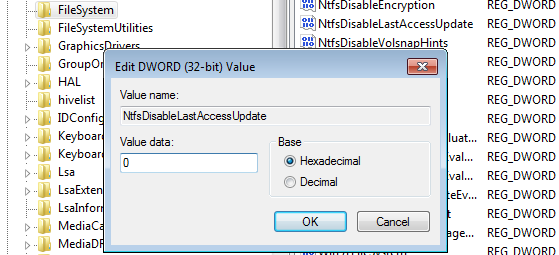
\includegraphics[scale=0.25]{images/lastAccess.png}
                \item Performance reasons
                \item Good for file server
            \end{itemize}
            \item Still updated some times
            \begin{itemize}
                \item File new created
                \item File copied
                \item File moved
            \end{itemize}
        \end{itemize}
    \end{itemize}
\end{frame}


\begin{frame}[fragile]
  \frametitle{5.4 Time Line: Exercise}
  \begin{lstlisting}[basicstyle=\tiny]
Reproduce file system activities
--------------------------------
  
     Thu Jun 27 2013 12:23:08      113 ...b         35-128-1 c:/time-01.txt
     Thu Jun 27 2013 12:24:20       75 m.cb         37-128-1 c:/time-02.txt
     Thu Jun 27 2013 12:25:24       75 m.cb         38-128-1 c:/time-03.txt
                                    75 m...         41-128-1 c:/time-03 - Copy.txt
     Thu Jun 27 2013 12:26:05       75 m..b         39-128-1 c:/time-44.txt
     Thu Jun 27 2013 12:27:00       75 macb         40-128-1 c:/time-05.txt (deleted)
     Thu Jun 27 2013 12:33:50      113 m.c.         35-128-1 c:/time-01.txt
     Thu Jun 27 2013 13:07:52       75 .acb         41-128-1 c:/time-03 - Copy.txt
     Thu Jun 27 2013 13:10:36       75 ..c.         39-128-1 c:/time-44.txt
     Thu Jun 27 2013 13:14:20       20 m...         42-128-1 c:/time-06.txt
     Thu Jun 27 2013 13:56:30       20 .acb         42-128-1 c:/time-06.txt


File: time-01.txt
-----------------
     Thu Jun 27 2013 12:23:08      113 ...b         35-128-1 c:/time-01.txt
     Thu Jun 27 2013 12:33:50      113 m.c.         35-128-1 c:/time-01.txt


File: time-02.txt
-----------------
     Thu Jun 27 2013 12:24:20       75 m.cb         37-128-1 c:/time-02.txt


-----
  \end{lstlisting}
\end{frame}


\begin{frame}[fragile]
  \frametitle{5.4 Time Line: Exercise}
  \begin{lstlisting}[basicstyle=\tiny]
Reproduce file system activities
--------------------------------
  
     Thu Jun 27 2013 12:23:08      113 ...b         35-128-1 c:/time-01.txt
     Thu Jun 27 2013 12:24:20       75 m.cb         37-128-1 c:/time-02.txt
     Thu Jun 27 2013 12:25:24       75 m.cb         38-128-1 c:/time-03.txt
                                    75 m...         41-128-1 c:/time-03 - Copy.txt
     Thu Jun 27 2013 12:26:05       75 m..b         39-128-1 c:/time-44.txt
     Thu Jun 27 2013 12:27:00       75 macb         40-128-1 c:/time-05.txt (deleted)
     Thu Jun 27 2013 12:33:50      113 m.c.         35-128-1 c:/time-01.txt
     Thu Jun 27 2013 13:07:52       75 .acb         41-128-1 c:/time-03 - Copy.txt
     Thu Jun 27 2013 13:10:36       75 ..c.         39-128-1 c:/time-44.txt
     Thu Jun 27 2013 13:14:20       20 m...         42-128-1 c:/time-06.txt
     Thu Jun 27 2013 13:56:30       20 .acb         42-128-1 c:/time-06.txt


File: time-03.txt, time-03 - Copy.txt
-------------------------------------
     Thu Jun 27 2013 12:25:24       75 m.cb         38-128-1 c:/time-03.txt
				    75 m...         41-128-1 c:/time-03 - Copy.txt
     Thu Jun 27 2013 13:07:52       75 .acb         41-128-1 c:/time-03 - Copy.txt


File: time-02.txt
-----------------
     Thu Jun 27 2013 12:26:05       75 m..b         39-128-1 c:/time-44.txt
     Thu Jun 27 2013 13:10:36       75 ..c.         39-128-1 c:/time-44.txt
-----
  \end{lstlisting}
\end{frame}


\begin{frame}[fragile]
  \frametitle{5.4 Time Line: Exercise}
  \begin{lstlisting}[basicstyle=\tiny]
Reproduce file system activities
--------------------------------
  
     Thu Jun 27 2013 12:23:08      113 ...b         35-128-1 c:/time-01.txt
     Thu Jun 27 2013 12:24:20       75 m.cb         37-128-1 c:/time-02.txt
     Thu Jun 27 2013 12:25:24       75 m.cb         38-128-1 c:/time-03.txt
                                    75 m...         41-128-1 c:/time-03 - Copy.txt
     Thu Jun 27 2013 12:26:05       75 m..b         39-128-1 c:/time-44.txt
     Thu Jun 27 2013 12:27:00       75 macb         40-128-1 c:/time-05.txt (deleted)
     Thu Jun 27 2013 12:33:50      113 m.c.         35-128-1 c:/time-01.txt
     Thu Jun 27 2013 13:07:52       75 .acb         41-128-1 c:/time-03 - Copy.txt
     Thu Jun 27 2013 13:10:36       75 ..c.         39-128-1 c:/time-44.txt
     Thu Jun 27 2013 13:14:20       20 m...         42-128-1 c:/time-06.txt
     Thu Jun 27 2013 13:56:30       20 .acb         42-128-1 c:/time-06.txt


File: time-05.txt
-----------------
     Thu Jun 27 2013 12:27:00       75 macb         40-128-1 c:/time-05.txt (deleted)


File: time-06.txt
-----------------
     Thu Jun 27 2013 13:14:20       20 m...         42-128-1 c:/time-06.txt
     Thu Jun 27 2013 13:56:30       20 .acb         42-128-1 c:/time-06.txt


-----
  \end{lstlisting}
\end{frame}


\begin{frame}[fragile]
  \frametitle{5.4 Time Line: Exercise}
  \begin{lstlisting}[basicstyle=\tiny]
Summary: What could we reproduce                                       Yes/No
-----------------------------------------------------------------------------
  
File: time-01.txt
      1. 12:23:08 time-01.txt -> new create                            Yes
      6. 12:29:07 time-01.txt -> modified content                          No
      7. 12:33:50 time-01.txt -> 2nd modification                      Yes

time-02.txt
      2. 12:24:20 time-02.txt -> new create                            Yes
      8. 12:29:50 time-02.txt -> open/access file                          No
      9. 12:30:01 time-02.txt -> close                                     No

time-03.txt, time-03 - Copy.txt
      3. 12:25:24 time-03.txt -> new create                            Yes
     10. 13:07:52 time-03.txt -> copy to time-0003 - Copy.txt          Yes/No

time-44.txt
      4. 12:26:05 time-04.txt -> new create                            Yes
     11. 13:10:36 time-04.txt -> rename to time-0044.txt               Yes/No

time-05.txt
      5. 12:27:00 time-05.txt -> new create                            Yes
     14. 13:58:07 time-05.txt -> delete file                               No

time-06.txt
     12. 13:14:20 time-06.txt -> new created on other drive            Yes/No
     13. 13:56:30 time-06.txt -> copy to local drive                   Yes
  \end{lstlisting}
\end{frame}


\begin{frame}[fragile]
\frametitle{5.5 Create a Time Line}
  \begin{lstlisting}[basicstyle=\tiny]
$ mkdir time


$ fls -f ntfs -o 2048 -m D:/ -r ntfs.raw > time/d.body

          -m    Time machine format
	  D:/   Add D:/ as mountpoint in report
          -r    Recursive


$ cd time
$ mactime -b d.body > d.time
$ less d.time

.....
Mon Dec 02 2019 16:25:22    15000 .a.b      73-128-2 D:/small_text_file.txt (deleted)
Wed Dec 04 2019 14:41:27    15051 .a.b      64-128-2 D:/AaaA.txt
Wed Dec 04 2019 14:42:06    15051 m.c.      64-128-2 D:/AaaA.txt
Wed Dec 04 2019 14:43:20    15000 macb      65-128-2 D:/Nonresident.txt (deleted)
Thu Dec 05 2019 12:10:53    24064 m.cb      66-128-2 D:/6-cluster.txt
Thu Dec 05 2019 12:11:12    24064 .a..      66-128-2 D:/6-cluster.txt
Mon Dec 09 2019 14:37:09      168 ...b      72-144-2 D:/NTFS_Sub_Dir
Mon Dec 09 2019 14:38:08      168 m.c.      72-144-2 D:/NTFS_Sub_Dir
                               13 macb      74-128-2 D:/NTFS_Sub_Dir/sub_Dir_File1.txt
Mon Dec 09 2019 14:38:24      168 .a..      72-144-2 D:/NTFS_Sub_Dir
Mon Dec 09 2019 16:09:46    15000 m.c.      73-128-2 D:/small_text_file.txt (deleted)
Sun Nov 29 2076 09:54:34    76800 macb       0-128-1 D:/$MFT
  \end{lstlisting}
\end{frame}





%
% This work is licensed under a Creative Commons Attribution-ShareAlike 4.0 International License.
% http://creativecommons.org/licenses/by-sa/4.0/
%

% DO NOT COMPILE THIS FILE DIRECTLY!
% This is included by the other .tex files.

%
% Reserved for EXT2, EXT3, EXT4 file systems
%

\begin{frame}
    
\includegraphics[scale=0.3]{images/logo-circl-Forensics.png}
    \begin{itemize}
        \item[]
        \item[]
        \item[] 6. 
    \end{itemize}
\end{frame}



%
% This work is licensed under a Creative Commons Attribution-ShareAlike 4.0 International License.
% http://creativecommons.org/licenses/by-sa/4.0/
%

% DO NOT COMPILE THIS FILE DIRECTLY!
% This is included by the other .tex files.


\begin{frame}
    
\includegraphics[scale=0.3]{images/logo-circl-Forensics.png}
    \begin{itemize}
        \item[]
        \item[]
        \item[] 7. Carving and String Search
    \end{itemize}
\end{frame}


\begin{frame}[fragile]
  \frametitle{7.1 Magic Bytes - File signatures}
  \begin{lstlisting}[basicstyle=\tiny]
xxd logo_h4k-350x250.jpg | less
0000000: ffd8 ffe0 0010 4a46 4946 0001 0100 0001  ......JFIF......
...
...
0008cc0: 0fa5 0a28 141a 0028 a0d0 3a50 07ff d9    ...(...(..:P...




xxd cases.jpg | less
0000000: ffd8 ffe1 0018 4578 6966 0000 4949 2a00  ......Exif..II*.
...
...
0001730: 4028 0500 a014 0280 501f ffd9            @(......P...




/etc/scalpel/scalpel.conf
-------------------------

   jpg     y     200000000     \xff\xd8\xff\xe0\x00\x10     \xff\xd9
   jpg     y     200000000     \xff\xd8\xff\xe1             \xff\xd9

  \end{lstlisting}
\end{frame}


\begin{frame}[fragile]
  \frametitle{7.1 Magic Bytes - File signatures}
  \begin{lstlisting}[basicstyle=\tiny]
xxd MECO-SMILE.pdf | less
0000000: 2550 4446 2d31 2e34 0a25 c7ec 8fa2 0a35  %PDF-1.4.%.....5
...
...
005c4d0: 3431 390a 2525 454f 460a                 419.%%EOF.




xxd LU-NCSS-2-EN.pdf | less
00000000: 2550 4446 2d31 2e35 0d25 e2e3 cfd3 0d0a  %PDF-1.5.%......
...
...
0007a7e0: 6566 0d31 3136 0d25 2545 4f46 0d         ef.116.%%EOF.




/etc/scalpel/scalpel.conf
-------------------------

   pdf     y       5000000     %PDF     %EOF\x0d     REVERSE
   pdf     y       5000000     %PDF     %EOF\x0a     REVERSE

  \end{lstlisting}
\end{frame}


\begin{frame}[fragile]
  \frametitle{7.2 Carving tools}
    \begin{itemize}
        \item Foremost
            \begin{itemize}
                \item Version 1.5.7
            \end{itemize}
        \item Scalpel
            \begin{itemize}
                \item Version 1.60
                \item Based on Foremost 0.69
            \end{itemize}
        \item Bulk Extractor
            \begin{itemize}
                \item Emails, Email addresses
                \item URLs
                \item Credit card numbers
                \item Social media
                \item Telephone numbers
                \item ...
            \end{itemize}
        \item Testdisk - Photorec
    \end{itemize}
\end{frame}


\begin{frame}[fragile]
  \frametitle{7.3 Limitations}
    \begin{itemize}
        \item Basically file system independent
        \item Data sequential
            \begin{itemize}
                \item Data must be sequential
                \item Fragmented data leads to broken files
                \item Very large files are more fragmented
                \item Depends on file system
                \item Depends on media type
                \item Data could be overwritten partially
            \end{itemize}
        \item End of file
            \begin{itemize}
                \item Does the file format support end marker
                \item Do we find a new magic byte
                \item Overlapping files
                \item Empty space at the end of a sector
            \end{itemize}
    \end{itemize}
\end{frame}


\begin{frame}[fragile]
  \frametitle{7.4 Exercise: Recover data from formated drive}
    \begin{itemize}
	\item Try meta data based recovery with \texttt{fls}
        \item Carving formated drive
        \begin{lstlisting}[basicstyle=\tiny]
mkdir out1/
foremost -t all -i formated.dd -o out1/

out1/audit.txt
--------------

File: deleted.dd
Start: Wed Aug 22 16:20:43 2018
Length: 32 MB (33554432 bytes)

Num      Name (bs=512)         Size      File Offset     Comment
0:      00009032.jpg           5 KB         4624384
1:      00009080.jpg          35 KB         4648960
2:      00037617.jpg          30 KB        19260232
3:      00037678.jpg         106 KB        19291633
.....
16:     00037608.pdf           1 MB        19255296
17:     00041288.pdf         489 KB        21139456       (PDF is Linearized)
Finish: Wed Aug 22 16:20:43 2018
18 FILES EXTRACTED

jpg:= 9
png:= 6
pdf:= 3
        \end{lstlisting}
    \end{itemize}
\end{frame}


\begin{frame}[fragile]
  \frametitle{7.5 What is 'String Search'?}
    \begin{itemize}
       \item Not sophisticated
       \item Search for strings
            \begin{itemize}
                \item At least 4 characters long
                \item From any file: Text, binary, disk image
		\item Search for ASCII, Unicode, big/little endian
            \end{itemize}
       \item Search the disk image for known words
            \begin{itemize}
                \item Terms used in a secret document
                \item IBAN ot other banking details
                \item Email addresses or URLs
            \end{itemize}
       \item Search thrue all the blocks
            \begin{itemize}
                \item Allocated non sllocated blocks
                \item File slack and outside partition boundaries
            \end{itemize}
       \item Goal
            \begin{itemize}
                \item Proof that the data was there once
                \item Identify intresting data that are close
            \end{itemize}
    \end{itemize}
\end{frame}


\begin{frame}[fragile]
  \frametitle{7.6 Examples}
    \begin{itemize}
       \item Search for strings
            \begin{itemize}
		    \item \texttt{strings -a circl-dfir.dd | less}
            \end{itemize}
       \item Min-Len
            \begin{itemize}
		    \item \texttt{strings -a -n 10 circl-dfir.dd | less}
            \end{itemize}
       \item Unicode 16 bit little endian
            \begin{itemize}
		    \item \texttt{strings -a -n 10 -el circl-dfir.dd | less}
            \end{itemize}
       \item Unicode 16 bit big endian
            \begin{itemize}
		    \item \texttt{strings -a -n 10 -eb circl-dfir.dd | less}
            \end{itemize}
       \item Offset in decimal
            \begin{itemize}
		    \item \texttt{strings -a -n 10 -eb -td circl-dfir.dd | less}
            \end{itemize}
       \item grep for your search term
            \begin{itemize}
		    \item \texttt{strings -a -n 10 -td circl-dfir.dd | grep -i paula}
            \end{itemize}
    \end{itemize}
\end{frame}


\begin{frame}[fragile]
  \frametitle{7.7 Steps to do a String Search}
    \begin{enumerate}
       \item Identify block/cluster size
            \begin{itemize}
		\item[] \texttt{mmls, fsstat}
            \end{itemize}
       \item Search for the string and the offset
            \begin{itemize}
		\item[] \texttt{blkls | srch\_strings | grep }
            \end{itemize}
       \item Calculate block/cluster of the string
	    \begin{itemize}
		\item[] \texttt{xxxxxxxxxx / 4096 = yyyy}
            \end{itemize}
       \item Review block/cluster content
	    \begin{itemize}
		\item[] \texttt{blkcat}
            \end{itemize}
       \item Identify inode of the block/cluster
	    \begin{itemize}
		\item[] \texttt{ifind}
            \end{itemize}
       \item Identify associated file
	    \begin{itemize}
		\item[] \texttt{ffind}
            \end{itemize}
       \item Recover file
	    \begin{itemize}
		\item[] \texttt{icat}
		\item[] Or mount and copy file
            \end{itemize}
    \end{enumerate}
\end{frame}


\newcounter{saveenumi}
\newcommand{\seti}{\setcounter{saveenumi}{\value{enumi}}}
\newcommand{\conti}{\setcounter{enumi}{\value{saveenumi}}}
\resetcounteronoverlays{saveenumi}

\begin{frame}[fragile]
  \frametitle{7.8 Exercise: What about Paulas cat?}
    \begin{enumerate}
        \item Identify cluster size
        \begin{lstlisting}[basicstyle=\tiny]
mmls circl-dfir.dd

    1      Slot      Start        End          Length       Description
 000:  Meta      0000000000   0000000000   0000000001   Primary Table (#0)
 001:  -------   0000000000   0000002047   0000002048   Unallocated
 002:  000:000   0000002048   0004917247   0004915200   NTFS / exFAT (0x07)



fsstat -o 2048 circl-dfir.dd

     File System Type: NTFS
     Volume Serial Number: 7B6E5F9427919882
     OEM Name: NTFS    
     Volume Name: CIRCL-DFIR
     Version: Windows XP

     .....

     Sector Size: 512
     Cluster Size: 4096
     Total Cluster Range: 0 - 614398
     Total Sector Range: 0 - 4915198
        \end{lstlisting}
    \seti
    \end{enumerate}
\end{frame}


\begin{frame}[fragile]
  \frametitle{7.8 Exercise: What about Paulas cat?}
    \begin{enumerate}
        \conti
        \item Search for the string \texttt{'Paula'}
        \begin{lstlisting}[basicstyle=\tiny]
blkls -e -o 2048 circl-dfir.dd | strings -a -td | grep -i paula

     157342 Paula's cat is fat.........
     157370 Paula's cat is fat.........
     .....
     157510 Paula's cat is fat.........
     157538 Paula's cat is fat.........
        \end{lstlisting}

        \item Calculate cluster of the string
        \begin{lstlisting}[basicstyle=\tiny]
echo $((157342/4096))
     38

echo $((157538/4096))
     38
        \end{lstlisting}

        \item Review cluster content
        \begin{lstlisting}[basicstyle=\tiny]
blkcat -o 2048 circl-dfir2dd 38 | strings
     .....
     Paula's cat is fat.........
     Paula's cat is fat.........
     Paula's cat is fat.........
     .....
        \end{lstlisting}
    \seti
    \end{enumerate}
\end{frame}


\begin{frame}[fragile]
  \frametitle{7.8 Exercise: What about Paulas cat?}
    \begin{enumerate}
        \conti
        \item Identify inode of the cluster
        \begin{lstlisting}[basicstyle=\tiny]
ifind -o 2048 -d 38 circl-dfir.dd 
  0-128-1
        \end{lstlisting}

        \item Identify associated file
        \begin{lstlisting}[basicstyle=\tiny]
ffind -o 2048 circl-dfir.dd 0-128-1
  //$MFT
        \end{lstlisting}

        \item Recover file
        \begin{lstlisting}[basicstyle=\tiny]
icat -o 2048 circl-dfir.dd 0-128-1 > MFT
        \end{lstlisting}
    \end{enumerate}
    \begin{itemize}
        \item[] Exercise: Manual approach - Learn from errors
        \begin{lstlisting}[basicstyle=\tiny]
dd if=circl-dfir.dd bs=4096 skip=38 count=1 | xxd | less
dd if=circl-dfir.dd bs=4096 skip=$((2048 + 38)) count=1 | xxd | less
dd if=circl-dfir.dd bs=4096 skip=$((2048/8 + 38)) count=1 | xxd | less
        \end{lstlisting}
        \end{itemize}
\end{frame}




%
% This work is licensed under a Creative Commons Attribution-ShareAlike 4.0 International License.
% http://creativecommons.org/licenses/by-sa/4.0/
%

% DO NOT COMPILE THIS FILE DIRECTLY!
% This is included by the other .tex files.


\begin{frame}
    
\includegraphics[scale=0.3]{images/logo-circl-Forensics.png}
    \begin{itemize}
        \item[]
        \item[]
        \item[] 8. Forensics Challenges
    \end{itemize}
\end{frame}


\begin{frame}[fragile]
  \frametitle{8.1 NTFS - Resident file becomes Non-Resident}
  \begin{itemize}
    \item Situation:
    \begin{itemize}
      \item NTFS formated partition
      \item A small resident file
      \item[]
    \end{itemize}
    \item Challenge:
    \begin{itemize}
      \item Analyze MFT record
      \item Let the file grow
      \item Analyze MFT record
      \item Analyze data clusters
      \item Modify content of the file
      \item Analyze data clusters
      \item Analyze MFT record
      \item[]
    \end{itemize}
  \end{itemize}
\end{frame}


\begin{frame}[fragile]
  \frametitle{8.1 NTFS - Resident file becomes Non-Resident}
  \begin{lstlisting}[basicstyle=\tiny]
$ ls -l /cdrom/NTFS_Sub_Dir/sub_Dir_File1.txt 
     13 Dez  9 14:38 /cdrom/NTFS_Sub_Dir/sub_Dir_File1.txt


$ fls -r -o 2048 ntfs.raw | grep File1
     + r/r 74-128-2:	sub_Dir_File1.txt


$ istat -o 2048 ntfs.raw 74 
     Attributes:
     Type: $DATA (128-2)   Name: N/A   Resident   size: 13


$ dd if=ntfs.raw skip=$((2048 + 4*8 + 74*2)) count=2 | xxd | less
     00000000: 4649 4c45 3000 0300 0000 0000 0000 0000  FILE0...........
     00000010: 0100 0100 3800 0100 9801 0000 0004 0000  ....8...........
     .....
     00000170: 0000 0000 0000 0200 0d00 0000 1800 0000  ................
     00000180: 4865 6c6c 6f20 576f 726c 6421 0a00 0000  Hello World!....
     00000190: ffff ffff 0000 0000 0000 0000 0000 0000  ................


$ for x in {1..1000}; do echo -n "$x "; done >> /cdrom/NTFS_Sub_Dir/sub_Dir_File1.txt

$ less /cdrom/NTFS_Sub_Dir/sub_Dir_File1.txt
     Hello World!
     1 2 3 4 5 6 7 8 9 10 11 12 13 14 15 16 17 18 19 20 21
     .....
  \end{lstlisting}
\end{frame}


\begin{frame}[fragile]
  \frametitle{8.1 NTFS - Resident file becomes Non-Resident}
  \begin{lstlisting}[basicstyle=\tiny]
$ ls -l /cdrom/NTFS_Sub_Dir/sub_Dir_File1.txt 
     3906 Apr 24 14:39 /cdrom/NTFS_Sub_Dir/sub_Dir_File1.txt


$ fls -r -o 2048 ntfs.raw | grep File1
     + r/r 74-128-2:	sub_Dir_File1.txt


$ istat -o 2048 ntfs.raw 74
     Attributes:
     Type: $DATA (128-2)   Name: N/A   Non-Resident   size: 3906  init_size: 3906
     4173


$ dd if=ntfs.raw skip=$((2048 + 4173*8)) count=8 | xxd | less
     00000000: 4865 6c6c 6f20 576f 726c 6421 0a31 2032  Hello World!.1 2
     00000010: 2033 2034 2035 2036 2037 2038 2039 2031   3 4 5 6 7 8 9 1
     00000020: 3020 3131 2031 3220 3133 2031 3420 3135  0 11 12 13 14 15
     .....


$ dd if=ntfs.raw skip=$((2048 + 4*8 + 74*2)) count=2 | xxd | less
     000001a0: 420f 0000 0000 0000 2101 4d10 0020 3135  B.......!.M.. 15
     000001b0: ffff ffff 0000 0000 3820 3139 2032 3020  ........8 19 20
     000001c0: 3231 2032 3220 3233 2032 3420 3235 2032  21 22 23 24 25 2
     .....
     000003e0: 2031 3737 2031 3738 2031 3739 2031 3830   177 178 179 180
     000003f0: 2031 3831 2000 0000 ffff ffff 0000 d607   181 ...........
  \end{lstlisting}
\end{frame}


\begin{frame}[fragile]
  \frametitle{8.1 NTFS - Resident file becomes Non-Resident}
  \begin{lstlisting}[basicstyle=\tiny]
Update file content: What happen with MFT Record?
-------------------------------------------------


$ echo -n 'We modify the content of the file. What is updated:
           Cluster? MFT Record? We will see.' | dd of=/cdrom/
	   NTFS_Sub_Dir/sub_Dir_File1.txt bs=44 seek=2 conv=notrunc


$ fls -r -o 2048 ntfs.raw | grep File1
     + r/r 74-128-2:	sub_Dir_File1.txt


$ istat -o 2048 ntfs.raw 74
     4173


$ dd if=ntfs.raw skip=$((2048 + 4173*8)) count=8 | xxd | less
     00000040: 3231 2032 3220 3233 2032 3420 3235 2032  21 22 23 24 25 2
     00000050: 3620 3237 2032 3820 5765 206d 6f64 6966  6 27 28 We modif
     00000060: 7920 7468 6520 636f 6e74 656e 7420 6f66  y the content of
     .....

$ dd if=ntfs.raw skip=$((2048 + 4*8 + 74*2)) count=2 | xxd | less
     000001c0: 3231 2032 3220 3233 2032 3420 3235 2032  21 22 23 24 25 2
     000001d0: 3620 3237 2032 3820 3239 2033 3020 3331  6 27 28 29 30 31
     000001e0: 2033 3220 3333 2033 3420 3335 2033 3620   32 33 34 35 36 
     .....
  \end{lstlisting}
\end{frame}


\begin{frame}[fragile]
  \frametitle{8.2 File System Tunneling}
  \begin{itemize}
    \item Situation:
    \begin{itemize}
      \item NTFS formated partition
      \item A normal file from before
      \item[]
    \end{itemize}
    \item Challenge:
    \begin{itemize}
      \item Analyze timestamps
      \item Delete the file
      \item Copy a file with the same filename
      \item Analyze timestamps
      \item Discover the behavior
      \item[]
    \end{itemize}
  \end{itemize}
\end{frame}


\begin{frame}[fragile]
  \frametitle{8.2 File System Tunneling}
  \begin{lstlisting}[basicstyle=\tiny]
1. Analyze time stamps of a file on NTFS
----------------------------------------

$ ll /cdrom/AaaA.txt
     15051 Dez  4 14:42 /cdrom/AaaA.txt*

$ fls -o 2048 ntfs.raw | grep AaaA
     r/r 64-128-2:	AaaA.txt

$ istat -o 2048 ntfs.raw 64

     $STANDARD_INFORMATION Attribute Values:
     Created:   	2019-12-04 14:41:27.333050500 (CET)
     File Modified:	2019-12-04 14:42:06.235661600 (CET)
     MFT Modified:	2019-12-04 14:42:06.235661600 (CET)
     Accessed:   	2019-12-04 14:41:27.333050500 (CET)

     $FILE_NAME Attribute Values:
     Created:   	2019-12-04 14:41:27.333050500 (CET)
     File Modified:	2019-12-04 14:41:27.333050500 (CET)
     MFT Modified:	2019-12-04 14:41:27.333050500 (CET)
     Accessed:  	2019-12-04 14:41:27.333050500 (CET)


2. Delete a file and create a new one with same filename
------------------------------------------
     # Do something like this on a Windows PC
     $ rm /cdrom/AaaA.txt; cp data_un.dd /cdrom/AaaA.txt
  \end{lstlisting}
\end{frame}


\begin{frame}[fragile]
  \frametitle{8.2 File System Tunneling}
  \begin{lstlisting}[basicstyle=\tiny]
3. Analyze time stamps of the new file
--------------------------------------

$ ll /cdrom/AaaA.txt 
     16384 Apr 27 15:51 /cdrom/AaaA.txt*


$ fls -o 2048 ntfs.raw | grep AaaA
     r/r 64-128-2:	AaaA.txt


$ istat -o 2048 ntfs.raw 64

     $STANDARD_INFORMATION Attribute Values:
     Created:   	2019-12-04 14:41:27.333050500 (CET)
     File Modified:	2019-12-04 14:42:06.235661600 (CET)
     MFT Modified:	2019-12-04 14:42:06.235661600 (CET)
     Accessed:  	2020-04-27 16:11:38.144645700 (CEST)

     $FILE_NAME Attribute Values:
     Created:   	2019-12-04 14:41:27.333050500 (CET)
     File Modified:	2019-12-04 14:41:27.333050500 (CET)
     MFT Modified:	2019-12-04 14:41:27.333050500 (CET)
     Accessed:  	2019-12-04 14:41:27.333050500 (CET)

  
  
.....
  \end{lstlisting}
\end{frame}


\begin{frame}[fragile]
  \frametitle{8.3 Un-Delete a file}
  \begin{itemize}
    \item Situation:
    \begin{itemize}
      \item NTFS formated partition
      \item A file is deleted
      \item[]
    \end{itemize}
    \item Challenge:
    \begin{itemize}
      \item Analyze MFT record before delete
      \item Analyze \$BITMAP file before delete
      \item Undo the modifications
      \item Analyze MFT record after undo
      \item Analyze \$BITMAP file after undo
      \item What is missing
      \item[]
    \end{itemize}
  \end{itemize}
\end{frame}


\begin{frame}[fragile]
  \frametitle{8.3 Un-Delete a file}
  \begin{lstlisting}[basicstyle=\tiny]
$ ls -l /cdrom/

  
$ fls -o 2048 ntfs.raw 
     -/r * 73-128-2:	small_text_file.txt


$ istat -o 2048 ntfs.raw 73
     Type: $DATA (128-2)   Name: N/A   Non-Resident   size: 15000  init_size: 15000
     4169 4170 4171 4172
  

Data cluster:
$ dd if=ntfs.raw skip=$((2048 + 4169*8)) count=$((4*8)) | xxd | less
 

MFT record 73: 
$ dd if=ntfs.raw skip=$((2048 + 4*8 + 73*2)) count=2| xxd | less


$Bitmap file
4169 / 8 = 521.125  --> Byte 521 (0x209) in $Bitmap file for Cluster 4168 - 4175
                    --> _ _ _ _  _ _ _ _
		              x  x x x   

$ icat -o 2048 ntfs.raw 6  | xxd | less
  \end{lstlisting}
\end{frame}


\begin{frame}[fragile]
  \frametitle{8.3 Un-Delete a file}
  \begin{lstlisting}[basicstyle=\tiny]
Fix $Bitmap file:
-----------------

$ istat -o 2048 ntfs.raw 6
     Type: $DATA (128-1)   Name: N/A   Non-Resident   size: 4064  init_size: 4064
     4071


$ dd if=ntfs.raw skip=$((2048 + 4071*8)) count=8 | xxd | less
     00000200: ffff ffff ffff ffff ffe1 0700 0000 0000  ................


4169 / 8 = 521.125  --> Byte 521 (0x209) in $Bitmap file for Cluster 4168 - 4175
                    --> _ _ _ _  _ _ _ _
		              x  x x x   
                        1 1 1 0  0 0 0 1
		    --> 1 1 1 1  1 1 1 1


$ dd if=ntfs.raw skip=$((2048 + 4071*8)) count=8 of=bitmap.dd
$ hexedit of=bitmap.dd
$ dd if=bitmap.dd seek=$((2048 + 4071*8)) of=ntfs.raw conv=notrunc


$ dd if=ntfs.raw skip=$((2048 + 4071*8)) count=8 | xxd | less
     00000200: ffff ffff ffff ffff ffff 0700 0000 0000  ................
  \end{lstlisting}
\end{frame}


\begin{frame}[fragile]
  \frametitle{8.3 Un-Delete a file}
  \begin{lstlisting}[basicstyle=\tiny]
Fix the MFT record:
-------------------

$ dd if=ntfs.raw skip=$((2048 + 4*8 + 73*2)) count=2 of=mft_73.dd


$ hexedit mft_73.dd
     00000000   46 49 4C 45  30 00 03 00  00 00 00 00  00 00 00 00  FILE0...........
     00000010   02 00 00 00  38 00 00 00  B8 01 00 00  00 04 00 00  ....8...........


      offset:     size:  old value:  new value:   description:
     ----------------------------------------------------------------------
         0010         2           2           1   Record sequence number
         0012         2           0           1   Link count
         0016         2           0           1   Record flag: 0000 = file deleted
                                                               0100 = file in use
         0030         2        1400               FixUp values
         03fe         2        1400               CRC


     00000000   46 49 4C 45  30 00 03 00  00 00 00 00  00 00 00 00  FILE0...........
     00000010   01 00 01 00  38 00 01 00  B8 01 00 00  00 04 00 00  ....8...........


$ dd if=mft_73.dd seek=$((2048 + 4*8 + 73*2)) count=2 of=ntfs.raw conv=notrunc
  \end{lstlisting}
\end{frame}


\begin{frame}[fragile]
  \frametitle{8.3 Un-Delete a file}
  \begin{itemize}
    \item What is missing?
    \begin{itemize}
      \item Compare output \texttt{ils} and \texttt{fls}
      \item What about the directory
      \item What is changed in a directory if a file is deleted?
      \item[]
    \end{itemize}
    \item[] $\to$ Forensics Hackathon
  \end{itemize}
\end{frame}






%
% This work is licensed under a Creative Commons Attribution-ShareAlike 4.0 International License.
% http://creativecommons.org/licenses/by-sa/4.0/
%

% DO NOT COMPILE THIS FILE DIRECTLY!
% This is included by the other .tex files.


\begin{frame}
    
\includegraphics[scale=0.3]{images/logo-circl-Forensics.png}
    \begin{itemize}
        \item[]
        \item[]
        \item[] 10. Bibliography and Outlook
    \end{itemize}
\end{frame}


\begin{frame}[fragile]
  \frametitle{10. Bibliography}
  \begin{itemize}
      \item Digital Forensics with Kali Linux
        \begin{itemize}
            \item[] Shiva V.N. Parasram
            \item[] Packt Publishing
            \item[] ISBN-13: 978-1-78862-500-5
        \end{itemize}
      \item[]
      \item Practical Forensic Imaging
        \begin{itemize}
            \item[] Bruce Nikkel
            \item[] No Starch Press
            \item[] ISBN-13: 978-1-59-327793-2
        \end{itemize}
      \item[]
      \item Digital Forensics with Open Source Tools
        \begin{itemize}
            \item[] Cory Altheide, Harlan Carvey
            \item[] Syngress
            \item[] ISBN-13: 978-1-59-749586-8
        \end{itemize}
  \end{itemize}
\end{frame}


\begin{frame}
  \frametitle{10. Bibliography}
  \begin{itemize}
      \item File System Forensic Analysis
        \begin{itemize}
            \item[] Brian Carrier
            \item[] Pearson Education
            \item[] ISBN-13: 978-0-32-126817-4
        \end{itemize}
      \item[]
      \item Forensic Computing: A Practitioner’s Guide
        \begin{itemize}
            \item[] Anthony Sammes, Brian Jenkinson
            \item[] Springer
            \item[] ISBN-13: 978-1-85-233299-0
        \end{itemize}
      \item[]
      \item[] 
        \begin{itemize}
            \item[]
            \item[]
            \item[] 
        \end{itemize}
  \end{itemize}
\end{frame}


\begin{frame}
  \frametitle{10. Outlook}
  \begin{itemize}
      \item[] CIRCL DFIR 1.0.2
      \begin{itemize}
          \item[]
          \item[] EXT File System
          \item[]
      \end{itemize}
  \end{itemize}
\end{frame}



\begin{frame}
  \frametitle{Overview}
  \begin{itemize}
  \item[]
      \begin{enumerate}
          \item File System Analysis - Overview
          \item FAT - File Allocation Table
          \item NTFS - New Technology File System
          \item NTFS - Advanced
          \item File System Time Line
          \item Carving
          \item String Search
          \item Forensics Challenges
          \item Bibliography and Outlook
      \end{enumerate}
  \end{itemize}
\end{frame}

\end{document}

